\documentclass[10pt,preprint2]{aastex}
\usepackage[a4paper,asymmetric,left=0.75in,right=0.75in,top=0.75in,bottom=0.75in]{geometry}
\AtBeginDocument{\newgeometry{asymmetric,left=0.75in,right=0.75in,top=0.75in,bottom=0.75in}\hoffset=0pt\setlength{\columnsep}{0.3in}\pagestyle{fancy}\fancyhf{}\fancyhead[L]{\small ASTRON 128 Astronomy Data Science Laboratory}\fancyhead[R]{\small Lab 2}\fancyfoot[C]{\thepage}}
\usepackage{amsmath, amsfonts, amssymb}
\usepackage{hyperref}
\usepackage{graphicx}
\usepackage{tikz}
\usepackage{booktabs}
\usepackage{fancyhdr}
\setlength{\headheight}{11pt}
\addtolength{\topmargin}{-0.16pt}
\usepackage{float}
\usepackage{stfloats}
\usepackage{pdflscape}
\usepackage{placeins}
\usepackage{pdfpages}\usetikzlibrary{arrows.meta,positioning,fit,calc,shapes.geometric}

\makeatletter\def\frontmatter@abstractheading{}\makeatother
\renewcommand{\abstractname}{}

% TikZ styles for pipeline flowchart
\tikzset{
  flowbox/.style={rectangle, rounded corners=4pt, draw=black, thick,
                  fill=blue!10, text width=3.0cm, align=center,
                  minimum height=0.8cm, font=\small},
  decisionbox/.style={diamond, draw=black, thick, fill=orange!15,
                      text width=2.2cm, align=center, aspect=1.5,
                      font=\footnotesize},
  outputbox/.style={rectangle, draw=black, thick, fill=green!15,
                    text width=2.5cm, align=center, minimum height=0.8cm,
                    font=\small},
  arrow/.style={-{Stealth[length=6pt]}, thick},
}

\begin{document}

\title{Data-Driven Modeling of APOGEE Stellar Spectra}
\author{Jun Rui Ting \\ \today\vspace{-2.5\baselineskip}}

\begin{abstract}
We present a data-driven spectral model for APOGEE DR17 red giants, following the methodology of \citet{Ness2015}. Starting from 1886 stars across four APOGEE fields (M15, NGC~6791, K2\_C4\_168-21, 060+00), selected with quality cuts on SNR, surface gravity, effective temperature, and metallicity, we download and pseudo-continuum normalize their $H$-band spectra (8575 pixels, 15100--17000~\AA). A second-order polynomial model (``The Cannon'') is trained on a 942-star subset, yielding 188,650 free parameters (21 coefficients + 1 intrinsic scatter per pixel) with a training reduced $\chi^2_r = 0.998$. Cross-validation on 944 held-out stars achieves scatters of 62~K in $T_{\rm eff}$, 0.13~dex in $\log g$, 0.045~dex in [Fe/H], 0.045~dex in [Mg/Fe], and 0.044~dex in [Si/Fe], with negligible biases. Gradient spectra confirm that the model captures known absorption features: Mg~I and Si~I lines dominate their respective abundance gradients, while $T_{\rm eff}$ demonstrates broadband and molecular features. A Kiel diagram of the cross-validation sample, colored by fitted [Fe/H], recovers the red giant branch and red clump with the expected metallicity gradient, in good agreement with 6~Gyr MIST v2 isochrones. MCMC fitting of a mystery spectrum via PyMC NUTS yields $T_{\rm eff} = 4582 \pm 4$~K, $\log g = 1.99 \pm 0.01$, $[\mathrm{Fe/H}] = -0.61 \pm 0.004$, $[\mathrm{Mg/Fe}] = +0.32 \pm 0.005$, and $[\mathrm{Si/Fe}] = +0.21 \pm 0.005$, identifying an alpha-enhanced red-clump giant. The MCMC uncertainties are $\sim$10--15$\times$ smaller than cross-validation scatter, attributable to unmodelled pixel-to-pixel correlations from continuum systematics and line blending. A baseline neural network (two hidden layers, 4.5M parameters) trained on the same data achieves $\sim$1.5--2$\times$ larger scatter than The Cannon on all labels, demonstrating the value of the more physically motivated polynomial labels. Synthetic spectra generated from the trained model illustrate how metallicity changes and RGB evolutionary state produce distinct spectral signatures, and we discuss the effects of unresolved binaries on label inference.

\vspace{2.5\baselineskip}
\end{abstract}

%%% ---------------------------------------------------------------
\section{Introduction}
\label{sec:intro}
%%% ---------------------------------------------------------------

Determining the physical properties of stars from their spectra is a central problem in stellar astrophysics. Traditional spectroscopic pipelines such as ASPCAP \citep{GarciaPerez2016} fit synthetic model atmospheres to observed spectra, requiring detailed line lists, opacity calculations, and assumptions about stellar physics. While powerful, these approaches are computationally expensive and systematically limited by incompleteness in the underlying atomic and molecular data \citep{Holtzman2015}.

An alternative paradigm is a data-driven approach: rather than predicting spectra from first-principles physics, one learns the mapping between stellar labels and spectra empirically from a training set of stars whose labels are already known. The Cannon \citep{Ness2015} implements this idea by modeling the flux at each wavelength pixel as a low-order (2\textsuperscript{nd}-order) polynomial in the stellar labels, trained on a reference set with labels from an existing pipeline. Once trained, the model can be inverted to infer labels for new spectra by $\chi^2$ minimization, bypassing the need for synthetic spectra entirely.

We apply this methodology to spectra from the Apache Point Observatory Galactic Evolution Experiment (APOGEE; \citealt{Majewski2017}), a high-resolution ($R \sim 22{,}500$), near-infrared ($H$-band, 1.51--1.70~$\mu$m) spectroscopic survey that has observed hundreds of thousands of stars across the Milky Way as part of the Sloan Digital Sky Surveys \citep{Abdurrouf2022}. The $H$-band is advantageous for stellar astrophysics because it suffers less dust extinction than optical wavelengths and contains numerous diagnostic absorption features of key elements including Fe, Mg, Si, Al, Ca, and molecular bands such as CN and CO.

In this work, we (1) assemble a training set of 1886 red giants from four APOGEE DR17 fields; (2) download, bitmask, and pseudo-continuum normalize their spectra; (3) train a second-order polynomial Cannon model and validate it via cross-validation; (4) compare The Cannon against a neural network approach; (5) use the model to construct a Kiel diagram and compare with MIST stellar isochrones; (6) fit a mystery spectrum using Bayesian MCMC; and (7) generate synthetic spectra to explore metallicity and evolutionary effects. Figure~\ref{fig:pipeline} provides an overview of the analysis pipeline.

\begin{figure*}[t!]
  \centering
  \resizebox{\textwidth}{!}{%
  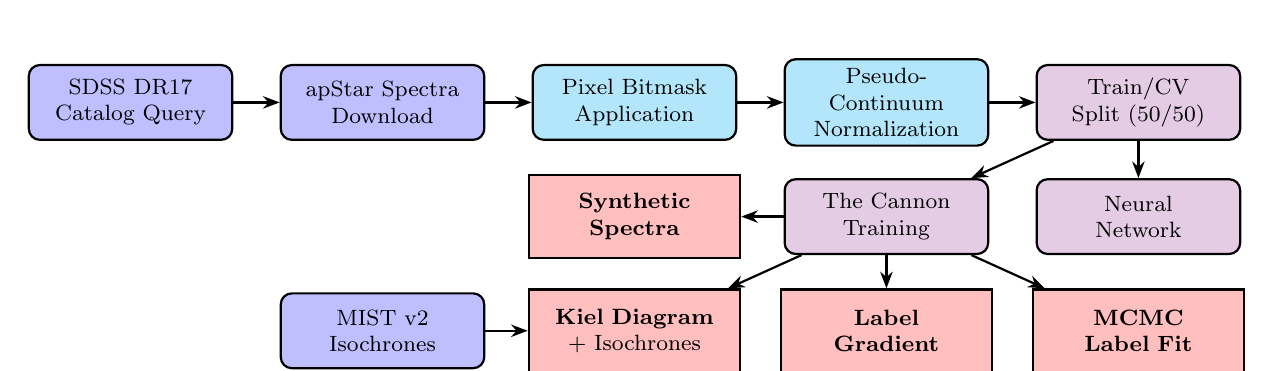
\begin{tikzpicture}[
    x=3.2cm,
    y=-1.45cm,
    pipebox/.style={flowbox, text width=2.35cm, minimum height=0.95cm, font=\footnotesize},
    pipeout/.style={outputbox, text width=2.45cm, minimum height=1.05cm, font=\footnotesize},
  ]
    % Row 0 (top): data acquisition — flows left to right
    \node[pipebox, fill=blue!25]   (query)     at (0,0) {SDSS DR17\\Catalog Query};
    \node[pipebox, fill=blue!25]   (download)  at (1,0) {apStar Spectra\\Download};
    \node[pipebox, fill=cyan!30]   (bitmask)   at (2,0) {Pixel Bitmask\\Application};
    \node[pipebox, fill=cyan!30]   (normalize) at (3,0) {Pseudo-Continuum\\Normalization};
    \node[pipebox, fill=violet!20] (split)     at (4,0) {Train/CV\\Split (50/50)};

    % Row 1: modelling — split branches to Cannon and NN; Synthetic Spectra from Cannon
    \node[pipeout, fill=red!25]    (synth)     at (2,1) {\textbf{Synthetic}\\{\textbf{Spectra}}};
    \node[pipebox, fill=violet!20] (train)     at (3,1) {The Cannon\\Training};
    \node[pipebox, fill=violet!20] (nn)        at (4,1) {Neural\\Network};

    % Row 2: results — remaining outputs from Cannon training
    \node[pipebox, fill=blue!25]   (mist)         at (1,2) {MIST v2\\Isochrones};
    \node[pipeout, fill=red!25]    (kiel)         at (2,2) {\textbf{Kiel Diagram}\\+ Isochrones};
    \node[pipeout, fill=red!25]    (gradient)     at (3,2) {\textbf{Label}\\{\textbf{Gradient}}};
    \node[pipeout, fill=red!25]    (mcmc)         at (4,2) {\textbf{MCMC}\\{\textbf{Label Fit}}};

    % Arrows — all connect direct neighbours
    % Row 0: left to right
    \draw[arrow] (query)     -- (download);
    \draw[arrow] (download)  -- (bitmask);
    \draw[arrow] (bitmask)   -- (normalize);
    \draw[arrow] (normalize) -- (split);

    % Split branches to both models (down-left and down)
    \draw[arrow] (split) -- (train);
    \draw[arrow] (split) -- (nn);

    % Cannon Training -> 4 results
    \draw[arrow] (train) -- (synth);
    \draw[arrow] (train) -- (gradient);
    \draw[arrow] (train) -- (mcmc);
    \draw[arrow] (train) -- (kiel);
    \draw[arrow] (mist)  -- (kiel);

  \end{tikzpicture}%
  }
  \caption{Analysis pipeline from APOGEE data acquisition to label inference. Node color indicates pipeline stage: \textcolor{blue!70!black}{Data Access} (catalog query and spectrum download); \textcolor{cyan!60!black}{Preprocessing} (bitmask application and pseudo-continuum normalization); \textcolor{violet}{Modeling} (train/CV split, Cannon training, neural network); \textcolor{red!60!black}{Key Results} (label gradient, Kiel diagram, synthetic spectra, MCMC label fit).}
  \label{fig:pipeline}
\end{figure*}

%%% ---------------------------------------------------------------
\section{Theoretical Background}
\label{sec:theory}
%%% ---------------------------------------------------------------

\subsection{Red Giants and the Kiel Diagram}

Red giants are evolved, luminous stars that have exhausted hydrogen in their cores and are burning hydrogen in a shell surrounding an inert (or, later, helium-burning) core. As a solar-mass star evolves off the main sequence, its envelope expands dramatically while the surface temperature decreases, tracing the red giant branch (RGB) in the Hertzsprung--Russell diagram.

Surface gravity $g = GM/R^2$ is a key diagnostic of evolutionary state. For a solar-mass star ($M = M_\odot$), the expected $\log g$ values at different evolutionary stages are:
\begin{align}
  \log g &= \log g_\odot + \log\!\left(\frac{M}{M_\odot}\right) - 2\log\!\left(\frac{R}{R_\odot}\right) \notag \\
         &= 4.44 - 2\log_{10}\!\left(\frac{R}{R_\odot}\right),
  \label{eq:logg}
\end{align}
where $\log g_\odot = 4.44$ in CGS units. Table~\ref{tab:logg_stages} shows how a log~$g$ cut at $\leq 4$ effectively separates giants ($R \gtrsim 2\,R_\odot$) from dwarfs.

\begin{table}[H]
\centering
\caption{Surface gravity at three evolutionary stages for a solar-mass star.\label{tab:logg_stages}}
\begin{tabular}{lcc}
\toprule
Stage & $R/R_\odot$ & $\log g$ \\
\midrule
Main sequence          & 1    & 4.44  \\
Pre-He flash (tip RGB) & 100  & 0.44  \\
Core He burning (red clump) & 15 & 2.09 \\
\bottomrule
\end{tabular}
\end{table}

The Kiel diagram plots $\log g$ vs.\ $T_{\rm eff}$ (with $T_{\rm eff}$ increasing leftward and $\log g$ decreasing upward, so that luminosity increases upward). In a sample of red giants, one expects to see the RGB as a diagonal running from hot, high-$\log g$ (base of the RGB) to cool, low-$\log g$ (tip), and the red clump as a dense concentration at $T_{\rm eff} \sim 4800$~K, $\log g \sim 2.5$ where core-helium-burning stars accumulate.

Metallicity modulates the RGB morphology. At lower [Fe/H], the envelope opacity decreases, stars are hotter at fixed luminosity, and the RGB shifts blueward. Isochrone models from MIST v2 \citep{Dotter2025} predict this shift quantitatively.

\subsection{The APOGEE Survey}

APOGEE \citep{Majewski2017} observes in the near-infrared $H$-band (15100--17000~\AA) at spectral resolution $R \sim 22{,}500$ using fiber-fed spectrographs with three Hawaii-2RG infrared detectors \citep{Wilson2019}. The three detector chips (blue, green, red) are resampled onto a common log-linear wavelength grid, producing a coadded spectrum of 8575 pixels per star.

APOGEE spectra are stored as \texttt{apStar} FITS files, one per star, containing the coadded (multi-visit combined) spectrum, associated error arrays, and a pixel-level quality bitmask (\texttt{APOGEE\_PIXMASK}). Since the Earth's orbital velocity ($\sim$30~km\,s$^{-1}$) causes a variable Doppler shift between visits, all individual visit spectra are shifted to a common Barycentric rest frame before coaddition \citep{Nidever2015}. This ensures that stellar absorption features appear at consistent wavelengths.

The aforementioned ASPCAP pipeline \citep{GarciaPerez2016} derives stellar labels ($T_{\rm eff}$, $\log g$, [Fe/H], and individual elemental abundances) by fitting synthetic model spectra to the observed data, which we use as our reference labels.

\subsection{Pseudo-Continuum Normalization}

Before modeling spectral features, the broadband spectral energy distribution (SED; a composition of the star's temperature, distance, and dust extinction) must be removed. True continuum normalization would divide by the stellar continuum (the spectrum in the absence of all absorption lines), which requires detailed knowledge of the atmospheric opacity. Instead, pseudo-continuum normalization fits a smooth function to wavelengths empirically identified as insensitive to label changes \citep{Ness2015}. The ratio of the observed spectrum to this smooth fit isolates the absorption/emission features as fractional deviations from unity.

Following \citet{Ness2015}, we use a set of 529 pre-identified continuum pixels\footnote{\url{https://github.com/ucb-datalab/course_materials_sp2026/tree/main/labs/lab_2}} distributed across the three APOGEE chips (241 blue, 108 green, 180 red). For each star and each chip independently, we fit a degree-4 Chebyshev polynomial to the flux at the continuum pixels, weighted by inverse variance. The full spectrum and error array are then divided by the chip's polynomial fit. Each chip receives its own independent polynomial to avoid artifacts at varying chip gaps.

\subsection{The Cannon: A Data-Driven Spectral Model}
\label{sec:cannon_theory}

The Cannon \citep{Ness2015} models the normalized flux at each wavelength pixel $\lambda$ as a function of the stellar label vector $\boldsymbol{\ell} = (T_{\rm eff}, \log g, [\mathrm{Fe/H}], [\mathrm{Mg/Fe}],$ $[\mathrm{Si/Fe}])$. Following \citet{Ness2015}, we adopt a second-order polynomial:
\begin{equation}
  f_{n\lambda} = \mathbf{X}_n \cdot \boldsymbol{\theta}_\lambda + \epsilon_{n\lambda},
  \label{eq:cannon_model}
\end{equation}
where $\mathbf{X}_n$ is the design vector for star $n$:
\begin{equation}
  \mathbf{X}_n = \bigl[1,\; \tilde{\ell}_1, \ldots, \tilde{\ell}_5,\; \tilde{\ell}_1^2, \tilde{\ell}_1\tilde{\ell}_2, \ldots, \tilde{\ell}_5^2\bigr],
  \label{eq:design_vector}
\end{equation}
with $\tilde{\ell}_i = (\ell_i - \mu_i)/\sigma_i$ being the centered and scaled labels (using training-set mean $\mu_i$ and standard deviation $\sigma_i$). This produces $\binom{5}{2} + 5 + 5 + 1 = 21$ terms: 1 constant, 5 linear, 10 cross-terms, and 5 quadratic. The vector $\boldsymbol{\theta}_\lambda$ contains the 21 model coefficients for pixel $\lambda$, and the noise $\epsilon_{n\lambda}$ follows $\mathcal{N}(0, \sigma_{n\lambda}^2 + s_\lambda^2)$, where $\sigma_{n\lambda}$ is the measurement uncertainty and $s_\lambda^2$ is the intrinsic scatter, defined as a per-pixel term that absorbs model inadequacy at wavelengths where a second-order polynomial is insufficient.

\subsubsection{Log-Likelihood and Training}

The log-likelihood for all training stars at pixel $\lambda$ is:
\begin{equation}
  \ln \mathcal{L}_\lambda = -\frac{1}{2}\sum_{n=1}^{N} \left[ \ln\bigl(2\pi(\sigma_{n\lambda}^2 + s_\lambda^2)\bigr) + \frac{(f_{n\lambda} - \mathbf{X}_n \cdot \boldsymbol{\theta}_\lambda)^2}{\sigma_{n\lambda}^2 + s_\lambda^2} \right].
  \label{eq:cannon_loglike}
\end{equation}
At fixed $s_\lambda^2$, the optimal coefficients are given by weighted least squares (WLS):
\begin{equation}
  \hat{\boldsymbol{\theta}}_\lambda(s_\lambda^2) = \left(\mathbf{X}^\top \mathbf{W}_\lambda \mathbf{X}\right)^{-1} \mathbf{X}^\top \mathbf{W}_\lambda \mathbf{f}_\lambda,
  \label{eq:wls}
\end{equation}
where $\mathbf{W}_\lambda = \mathrm{diag}\bigl((\sigma_{n\lambda}^2 + s_\lambda^2)^{-1}\bigr)$ and $\mathbf{X}$ is the $N \times 21$ design matrix. This makes training efficient: we solve analytically for $\boldsymbol{\theta}_\lambda$ at each candidate $s_\lambda^2$, then optimize over $\log s_\lambda^2$ via one-dimensional scalar minimization. Each of the 8575 pixels is trained independently.

\subsubsection{Label Fitting}

Given a trained model $\{\boldsymbol{\theta}_\lambda, s_\lambda^2\}$, we infer the labels of a new star by minimizing:
\begin{equation}
  \chi^2(\boldsymbol{\ell}) = \sum_\lambda \frac{\bigl(f_\lambda^{\rm obs} - \hat{f}_\lambda(\boldsymbol{\ell})\bigr)^2}{\sigma_\lambda^2 + s_\lambda^2},
  \label{eq:cannon_chi2}
\end{equation}
using the Trust Region Reflective (TRF) algorithm in \texttt{scipy.optimize.least\_squares}. Additionally, we compute the Jacobian $\partial\hat{f}_\lambda/\partial\ell_j$ analytically from the polynomial structure of the design vector.

\subsection{Bayesian MCMC Label Fitting}

For the mystery spectrum, we perform MCMC following a posterior:
\begin{equation}
  p(\boldsymbol{\ell} \mid \mathbf{f}) \propto p(\mathbf{f} \mid \boldsymbol{\ell})\, p(\boldsymbol{\ell}),
\end{equation}
where the log-likelihood for a single star with observed spectrum $\mathbf{f}$ is:
\begin{equation}
  \ln p(\mathbf{f} \mid \boldsymbol{\ell}) = -\frac{1}{2}\sum_{\lambda} \left[ \ln\bigl(2\pi(\sigma_\lambda^2 + s_\lambda^2)\bigr) + \frac{(f_\lambda - \hat{f}_\lambda(\boldsymbol{\ell}))^2}{\sigma_\lambda^2 + s_\lambda^2} \right],
  \label{eq:mcmc_loglike}
\end{equation}
summing over all wavelength pixels $\lambda$, with the predicted spectrum $\hat{f}_\lambda(\boldsymbol{\ell})$ and trained scatter $s_\lambda^2$ from the Cannon model. We adopt weakly informative Gaussian priors on each label:
\begin{equation}
  \ell_i \sim \mathcal{N}(\mu_i, (2\sigma_i)^2),
  \label{eq:priors}
\end{equation}
centered on the training-set mean with width twice the training-set standard deviation. This choice is motivated by the observation that the training-set label distributions are broadly Gaussian (Figure~\ref{fig:label_corner}); thus this choice of priors reflects a physically-sound range of label values. We sample the posterior using the No-U-Turn Sampler (NUTS; \citealt{HoffmanGelman2014}) as implemented in PyMC \citep{Salvatier2016}.

\subsection{Neural Network Label Prediction}
\label{sec:nn_theory}

As an alternative to the forward-model-then-invert approach of The Cannon, one can directly learn a mapping from spectra to labels using a neural network. We train a multi-layer perceptron (MLP) that takes a normalized 8575-pixel spectrum as input and predicts the 5-element label vector. This reverses the direction of inference: rather than modeling $f(\boldsymbol{\ell}) \to \mathrm{spectrum}$, the network learns $\mathrm{spectrum} \to \boldsymbol{\ell}$.

\subsubsection{Multi-Layer Perceptrons}

An MLP is a composition of alternating affine transformations and element-wise nonlinear activation functions \citep{Goodfellow2016}. A single layer maps an input vector $\mathbf{x} \in \mathbb{R}^{d_{\rm in}}$ to an output representation $\mathbf{h} \in \mathbb{R}^{d_{\rm out}}$ via:
\begin{equation}
  \mathbf{h} = \sigma\!\bigl(\mathbf{W}\mathbf{x} + \mathbf{b}\bigr),
  \label{eq:mlp_layer}
\end{equation}
where $\mathbf{W} \in \mathbb{R}^{d_{\rm output} \times d_{\rm input}}$ is a learnable weight matrix, $\mathbf{b} \in \mathbb{R}^{d_{\rm output}}$ is a bias vector, and $\sigma(\cdot)$ is a nonlinear activation function applied element-wise. Without the activation function, a stack of linear layers collapses to a single affine map ($\mathbf{W}_2 \mathbf{W}_1 = \mathbf{W}_{\rm eff}$), so the activation function's nonlinearity allows for linear layers to ``learn'' complex relationships.

A standard activation function is the Rectified Linear Unit (ReLU):
\begin{equation}
  \sigma(z) = \max(0, z),
  \label{eq:relu}
\end{equation}
which is computationally cheap compared to $\tanh$ or the logistic sigmoid, but introduces the piecewise-linear nonlinearity.

A complete MLP with two hidden layers (the architecture we adopt as our baseline) computes:
\begin{equation}
  \hat{\boldsymbol{\ell}} = \mathbf{W}_3 \,\sigma\!\bigl(\mathbf{W}_2 \,\sigma\!\bigl(\mathbf{W}_1 \mathbf{x} + \mathbf{b}_1\bigr) + \mathbf{b}_2\bigr) + \mathbf{b}_3,
  \label{eq:mlp_full}
\end{equation}
where the final layer has no activation, producing an unconstrained real-valued output suitable for regression. The total number of learnable parameters is $\sum_{k=1}^{L}(d_{k-1} + 1) \times d_k$, where $d_0$ is the input dimension and $d_L$ is the output dimension.

% The \textit{universal approximation theorem} \citep{Hornik1989} guarantees that a single hidden layer of sufficient width can approximate any continuous function on a compact set to arbitrary accuracy. In practice, moderate-depth networks (2--3 layers) with moderate width achieve better parameter efficiency than a single extremely wide layer, because depth enables hierarchical feature extraction: early layers learn local patterns (e.g., individual absorption line shapes) while later layers combine them into global predictions (e.g., stellar labels).

\subsubsection{Loss Functions and Optimizers}

The network is trained by minimizing a loss function over the training set. For regression, a standard choice is the mean squared error (MSE):
\begin{equation}
  \mathcal{L}_{\rm MSE} = \frac{1}{N}\sum_{n=1}^{N} \bigl\|\hat{\boldsymbol{\ell}}_n - \boldsymbol{\ell}_n\bigr\|^2,
  \label{eq:mse_loss}
\end{equation}
where the sum is over training stars.
% Minimizing MSE is equivalent to maximizing a Gaussian log-likelihood with constant, isotropic variance---analogous to The Cannon's $\chi^2$ fitting (Eq.~\ref{eq:cannon_chi2}) but without per-pixel heteroscedastic weights. This simplification means the network treats all pixels equally, giving undue weight to noisy pixels.
To ensure equal weighting across labels of different physical scales (i.e., K vs.\ dex), we normalize all labels to zero mean and unit variance before training.

The weight matrices $\mathbf{W}_k$ and biases $\mathbf{b}_k$ are learned by minimizing the MSE loss via gradient-based optimization. We use Adam \citep{Kingma2015}, which maintains per-parameter running estimates of the gradient's first and second moments and uses these to scale the learning rate adaptively.

\subsubsection{Regularization and Early Stopping}

With $\sim$4.5 million parameters trained on $\sim$940 spectra, overfitting is a persistent risk. Early stopping halts training when the validation loss stops improving, implicitly limiting model complexity by restricting how far parameters move from initialization. Dropout \citep{Srivastava2014} randomly zeroes a fraction $p$ of hidden activations each training step, preventing correlated adaptation of neurons. Weight decay (L2 regularization) adds a penalty $\lambda \|\mathbf{W}\|_F^2$ to the loss, shrinking weights toward zero and encouraging smoother learned functions. However, in the data-limited regime of this report ($N \sim 1000$), applying these strategies in tandem can harm performance when the network is already capacity-limited.

%%% ---------------------------------------------------------------
\section{Data Acquisition and Preparation}
\label{sec:data}
%%% ---------------------------------------------------------------

\subsection{Training Set Selection}

We queried the SDSS DR17 \texttt{apogeeStar} and \texttt{aspcapStar} catalogs via \texttt{astroquery} for stars in four APOGEE fields: M15, N6791 (NGC~6791), K2\_C4\_168-21, and 060+00. These fields span a wide range of stellar populations: M15 is a metal-poor halo globular cluster ($[\mathrm{Fe/H}] \sim -2.3$; \citealt{Harris1996}), NGC~6791 is a metal-rich open cluster ($[\mathrm{Fe/H}] \sim +0.3$; \citealt{Brogaard2012}), K2\_C4\_168-21 samples disk giants at intermediate metallicities, and 060+00 targets the inner disk and bulge.

We applied quality cuts to ensure reliable training labels:
\begin{itemize}
  \item All five ASPCAP labels ($T_{\rm eff}$, $\log g$, [Fe/H], [Mg/Fe], [Si/Fe]) finite and not equal to the ASPCAP null sentinel $-9999$.
  \item Signal-to-noise ratio $\mathrm{SNR} > 50$.
  \item $\log g \leq 4$ and $T_{\rm eff} \leq 5700$~K (selecting red giants; see Eq.~\ref{eq:logg} and Table~\ref{tab:logg_stages}).
  \item $[\mathrm{Fe/H}] \geq -1$ (excluding metal-poor stars where ASPCAP labels may be less reliable and the polynomial model may extrapolate poorly).
\end{itemize}
After these cuts, 1886 stars remain in the training set.

\begin{figure*}[t!]
  \centering
  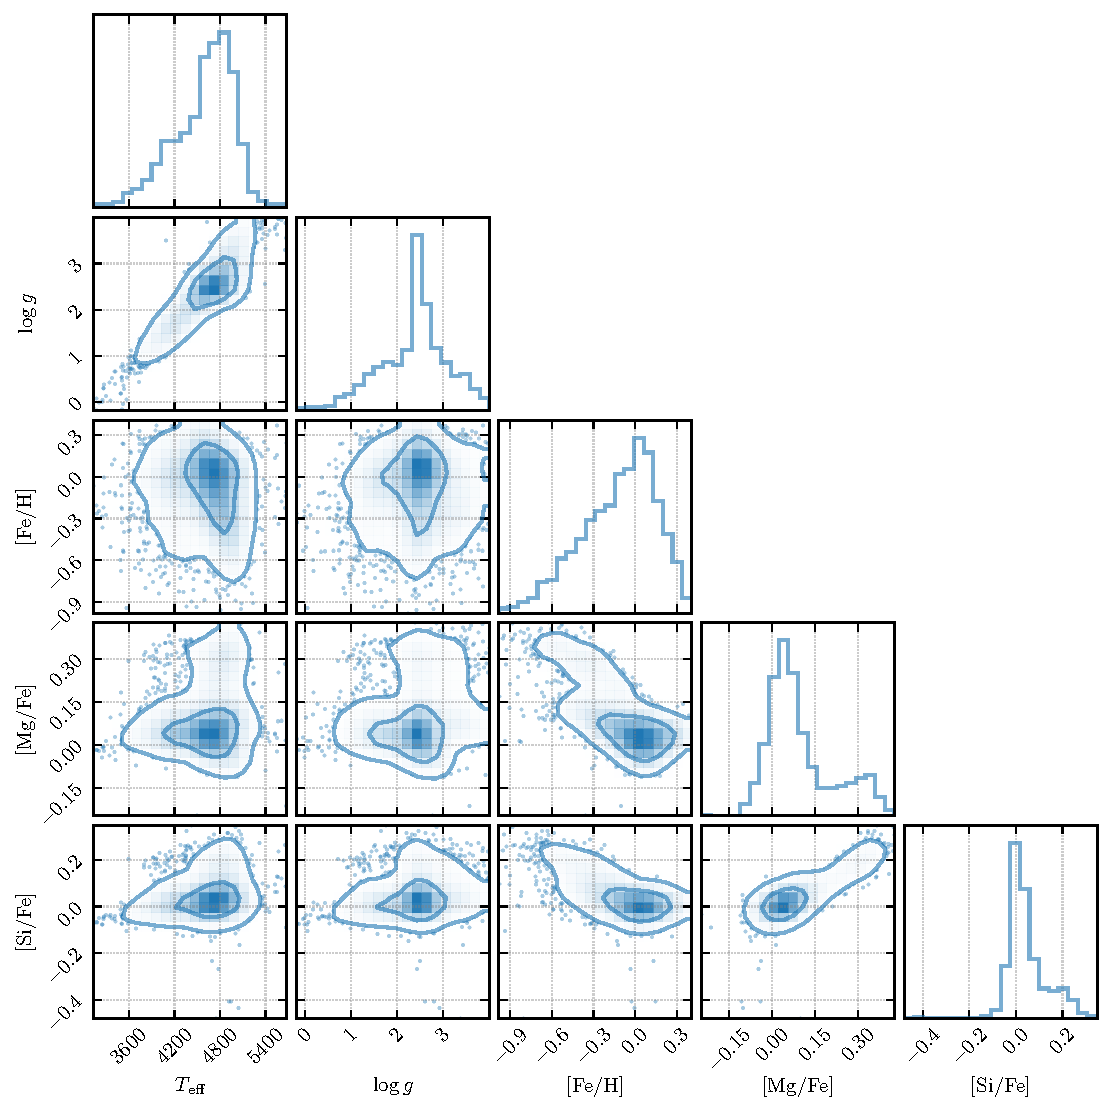
\includegraphics[width=\textwidth]{figures/fig_label_corner.pdf}
  \caption{Corner plot of the five ASPCAP labels for the 1886-star training set. The $T_{\rm eff}$--$\log g$ panel traces the red giant branch (diagonal locus) and red clump (dense concentration at $T_{\rm eff} \sim 4800$~K, $\log g \sim 2.5$). The [Mg/Fe]--[Si/Fe] panel shows a tight positive correlation, reflecting the common nucleosynthetic origin of $\alpha$-elements. The [Fe/H] marginal distribution is bimodal, reflecting the mixture of metal-poor (M15) and metal-rich (NGC~6791) cluster fields.}
  \label{fig:label_corner}
\end{figure*}

Figure~\ref{fig:label_corner} shows the distribution of the training set in the five-dimensional label space. The $T_{\rm eff}$--$\log g$ projection traces the expected red giant branch morphology with a dense red clump at $T_{\rm eff} \sim 4800$~K, $\log g \sim 2.5$. The tight positive correlation between [Mg/Fe] and [Si/Fe] reflects the common nucleosynthetic origin of $\alpha$-elements in core-collapse supernovae. The bimodal [Fe/H] distribution arises from the mixture of metal-poor (M15) and metal-rich (NGC~6791) cluster populations.

\subsection{Spectrum Download and Wavelength Reconstruction}

For each star, we downloaded the \texttt{apStar-dr17} FITS file from the SDSS data archive. The coadded spectrum (HDU~1, row~0), error array (HDU~2, row~0), and pixel bitmask (HDU~3, row~0) were extracted. The wavelength array was reconstructed from the FITS header using the log-linear WCS:
\begin{equation}
  \lambda_i = 10^{\texttt{CRVAL1} + \texttt{CDELT1} \times i}, \quad i = 0, 1, \ldots, 8574,
\end{equation}
spanning 15100.8--16999.8~\AA. The flux units are $10^{-17}$~erg\,s$^{-1}$\,cm$^{-2}$\,\AA$^{-1}$ (spectral flux density).

\subsection{Pixel Bitmask Application}

The \texttt{APOGEE\_PIXMASK} bitmask flags problematic pixels. Following the APOGEE data model documentation, we mask bits 0--7 and bit~12 (Table~\ref{tab:bitmask}).
\begin{table}[t]
\centering
\caption{APOGEE\_PIXMASK bits used for pixel masking.\label{tab:bitmask}}
\begin{tabular}{ccl}
\toprule
Bit & Name & Description \\
\midrule
0 & \texttt{BADPIX}     & Bad pixels \\
1 & \texttt{CRPIX}      & Cosmic ray hit \\
2 & \texttt{SATPIX}     & Saturated pixel \\
3 & \texttt{UNFIXABLE}  & Unfixable by reduction pipeline \\
4 & \texttt{BADDARK}    & Bad dark current subtraction \\
5 & \texttt{BADFLAT}    & Bad flat-field correction \\
6 & \texttt{BADERR}     & Unreliable error estimate \\
7 & \texttt{NOSKY}      & Sky subtraction failed \\
12 & \texttt{NODATA}    & No data (unvisited pixel) \\
\bottomrule
\end{tabular}
\end{table}
For bitmask-flagged pixels, we set the uncertainty to a large sentinel value ($\sigma = 10^6$), giving them negligible weight ($\sim 10^{-12}$) in any $\chi^2$-based fit. Pixels with NaN or negative flux (inter-chip gaps, sky over-subtraction) have both their flux and error set to NaN, which propagates through all downstream calculations and excludes them automatically. Across the 1886 training spectra, the mean masked fraction per star is 9.8\% (mean 839, median 826 of 8575 pixels per star).

Figure~\ref{fig:bitmask_diagnostic} shows a raw example spectrum with bitmask-flagged regions highlighted. Figure~\ref{fig:bitmask_frequency} shows the per-pixel mask frequency across all 1886 training spectra, revealing persistent masking patterns at chip edges and telluric-affected regions.

\begin{figure*}[t!]
  \centering
  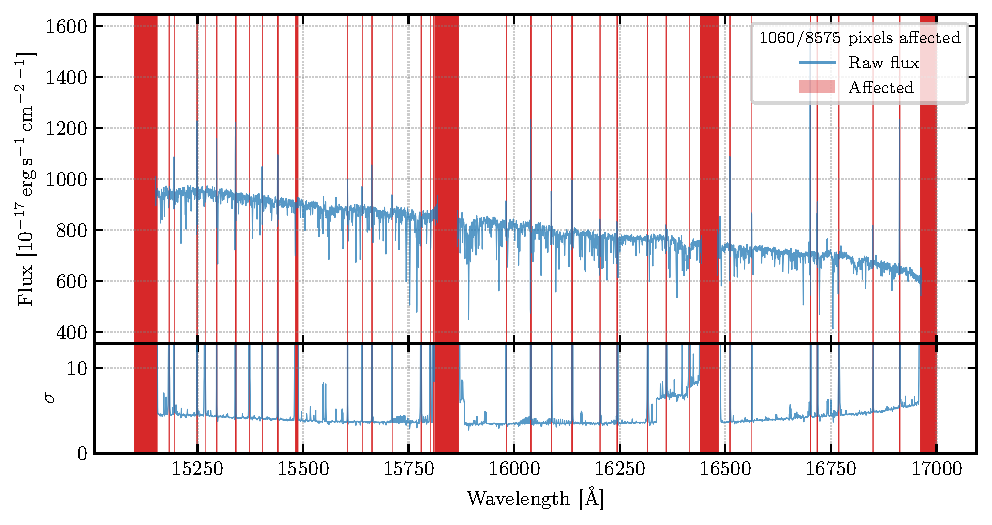
\includegraphics[width=\textwidth]{figures/fig_bitmask_diagnostic.pdf}
  \caption{Raw APOGEE DR17 spectrum of 2M21235315+1244123. \textit{Top:} Flux vs.\ wavelength showing the three detector chips (blue, green, red) with inter-chip gaps. Prominent absorption features include H~I Brackett series lines (Br11--Br20), CO bands ($\lambda > 15580$~\AA), and numerous metal lines (Fe~I, Mg~I, Si~I, Al~I, Ca~I). Red-shaded regions indicate bitmask-flagged pixels (Table~\ref{tab:bitmask}); common causes include persistence artifacts, cosmic ray hits, spurious emission lines, and sky subtraction residuals. \textit{Bottom:} Per-pixel uncertainty array.}
  \label{fig:bitmask_diagnostic}
\end{figure*}

\begin{figure*}[t!]
  \centering
  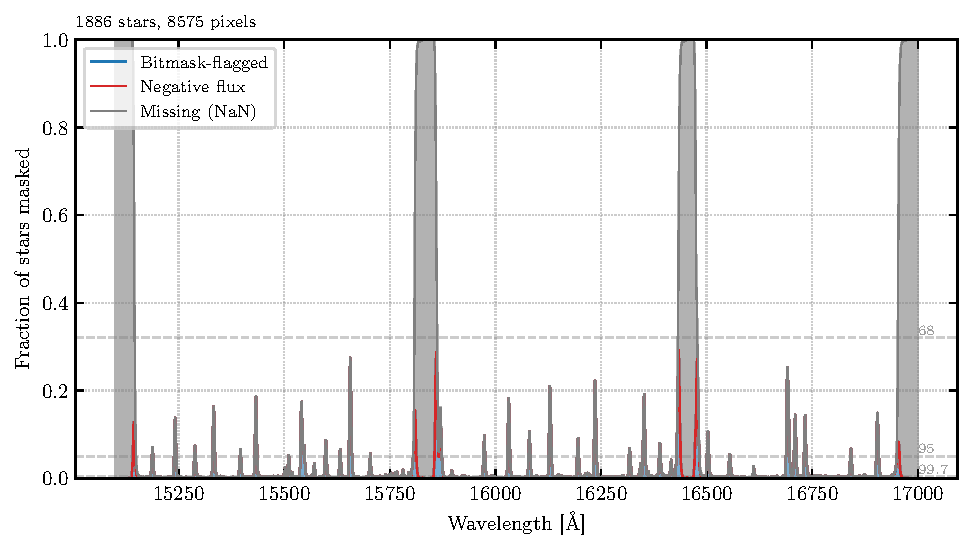
\includegraphics[width=\textwidth]{figures/fig_bitmask_frequency.pdf}
  \caption{Per-pixel mask frequency across all 1886 training spectra. The three APOGEE detector chips show distinct masking patterns: chip edges and persistence-affected regions have elevated mask rates, while the majority of pixels are flagged in fewer than 5\% of spectra.}
  \label{fig:bitmask_frequency}
\end{figure*}

\subsection{Pseudo-Continuum Normalization}

We normalize each spectrum chip-by-chip using the 529 pre-identified continuum pixels. For each of the three chips, we fit a degree-4 Chebyshev polynomial to the continuum pixels (those with finite errors and not flagged by the bitmask), weighted by inverse variance. The spectrum and error array are then divided by the polynomial fit.

Figure~\ref{fig:normalization} shows the normalization procedure for star 2M21235315+1244123; the raw spectrum with the per-chip Chebyshev continuum fits overlaid, and the resulting normalized spectrum.

\begin{figure*}[t!]
  \centering
  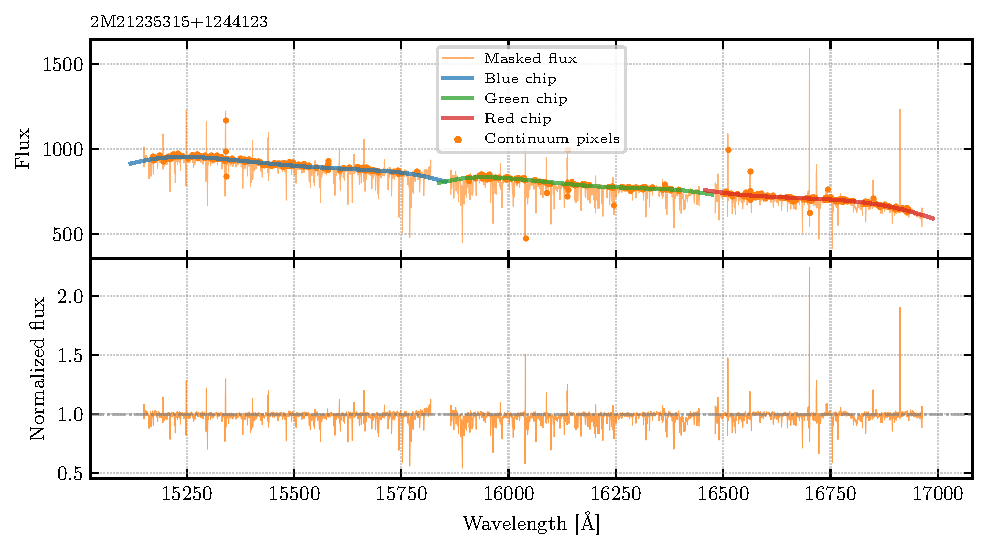
\includegraphics[width=\textwidth]{figures/fig_normalization.pdf}
  \caption{Pseudo-continuum normalization for 2M21235315+1244123. \textit{Top:} Masked raw spectrum (orange) with per-chip degree-4 Chebyshev continuum fits (colored curves); shaded bands indicate the 529 continuum pixels used to anchor the fits. \textit{Bottom:} Normalized spectrum, where the continuum level has been divided out and absorption features appear as deviations below unity.}
  \label{fig:normalization}
\end{figure*}

To verify normalization robustness, Figure~\ref{fig:similar_stars} compares the normalized spectra of stars with similar ASPCAP labels. If normalization is working correctly, stars with similar labels should have nearly identical normalized spectra. The median per-pixel scatter among 5 nearest neighbors in label space is $\sim$0.01 ($\sim$1\% of continuum), confirming that the normalization does not introduce significant artifacts.

\begin{figure*}[t!]
  \centering
  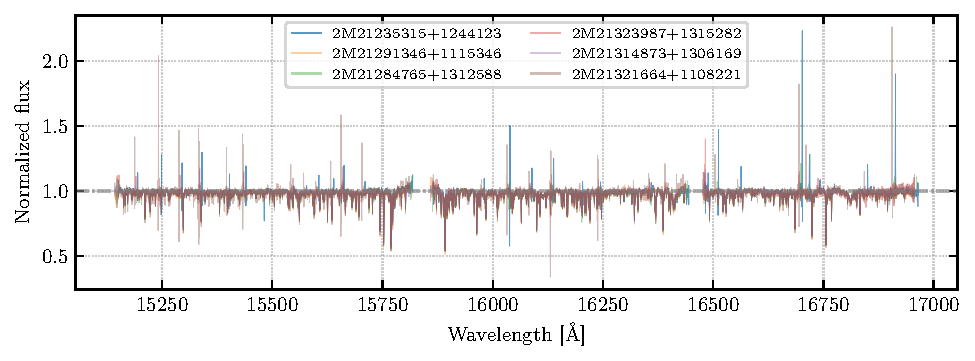
\includegraphics[width=\textwidth]{figures/fig_similar_stars.pdf}
  \caption{Normalization robustness check. \textit{Top:} Normalized spectra of 2M21235315+1244123 (blue) and its 5 nearest neighbors in label space (colored). \textit{Bottom:} Per-pixel standard deviation across the 6 spectra. The median scatter of $\sim$0.01 confirms that pseudo-continuum normalization does not introduce significant star-to-star artifacts at the percent level.}
  \label{fig:similar_stars}
\end{figure*}

%%% ---------------------------------------------------------------
\section{The Cannon}
\label{sec:cannon}\label{sec:training}
%%% ---------------------------------------------------------------

\subsection{Training and Cross-Validation Split}

We split the 1886-star sample into a training set (942 stars) and a cross-validation (CV) set (944 stars) using a stratified 50/50 random split whereby within each APOGEE field, half the stars are assigned to training and half to CV. This preserves the metallicity and evolutionary-state coverage in both subsets.

\begin{figure*}[t!]
  \centering
  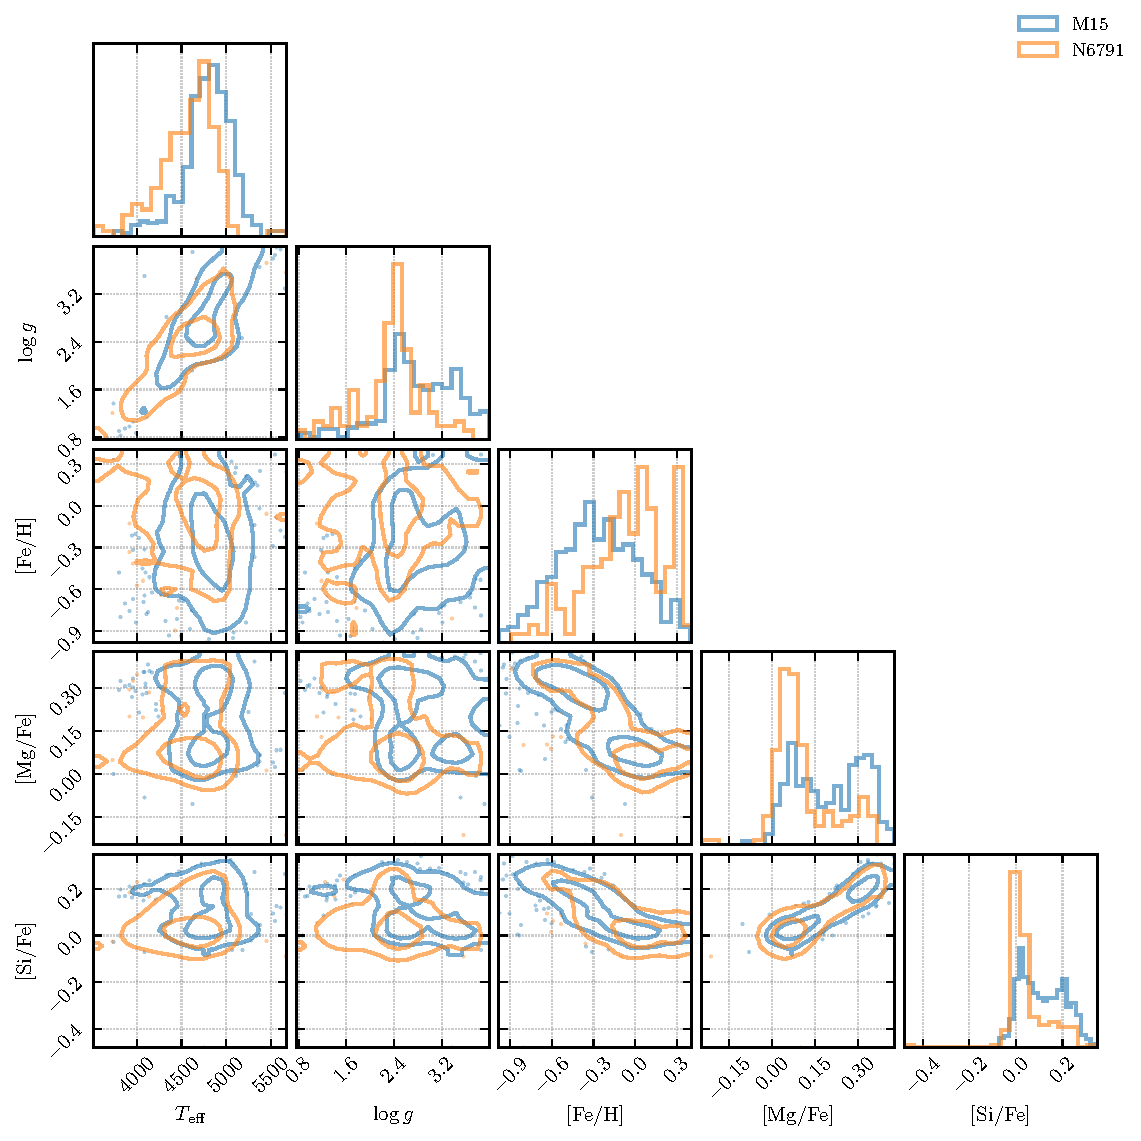
\includegraphics[width=\textwidth]{figures/fig_label_corner_by_field.pdf}
  \caption{Corner plot of stellar labels colored by APOGEE field. The stratified split preserves the label distributions of all four fields in both training and cross-validation subsets.}
  \label{fig:label_corner_by_field}
\end{figure*}

Figure~\ref{fig:label_corner_by_field} confirms that the training and CV subsets span the same regions of label space.
% Table~\ref{tab:split_sizes} gives the per-field breakdown.

% \begin{table}[H]
% \centering
% \caption{Training and cross-validation subset sizes by APOGEE field.\label{tab:split_sizes}}
% \begin{tabular}{lcc}
% \toprule
% Field & $N_{\rm train}$ & $N_{\rm CV}$ \\
% \midrule
% 060+00          & 444 & 444 \\
% K2\_C4\_168-21  & 141 & 142 \\
% M15             & 271 & 272 \\
% N6791           & 86  & 86  \\
% \midrule
% Total           & 942 & 944 \\
% \bottomrule
% \end{tabular}
% \end{table}

\subsection{Design Matrix Construction}

The design matrix $\mathbf{X}$ has shape $(942, 21)$. Labels are first centered and scaled to zero mean and unit variance as described. The 21 columns correspond to: $\bigl[1,\; T_{\rm eff},\; \log g,\; \mathrm{[Fe/H]},\; \mathrm{[Mg/Fe]},\; \mathrm{[Si/Fe]},\; T_{\rm eff}^2,\; T_{\rm eff}\!\cdot\!\log g,\; \ldots,\; \mathrm{[Si/Fe]}^2\bigr].$.
The model is mathematically equivalent to the unscaled formulation of \citet{Ness2015}; the scaling is absorbed into the $\boldsymbol{\theta}_\lambda$ coefficients.

Together, the total number of free parameters is $(21 + 1) \times 8575 = 188{,}650$ where each pixel contributes 21 polynomial coefficients and 1 scatter term.

\subsection{Training Results}

The training reduced $\chi^2_r$, computed as:
\begin{equation}
  \chi^2_r = \frac{1}{N_{\rm train}} \sum_{n=1}^{N_{\rm train}} \frac{1}{\nu_n} \sum_\lambda \frac{(f_{n\lambda} - \hat{f}_{n\lambda})^2}{\sigma_{n\lambda}^2 + s_\lambda^2},
\end{equation}
is $\chi^2_r = 0.998$, indicating that the model (including the scatter term) adequately describes the training data.

\subsection{Training Set Prediction Verification}

To confirm the model is functioning correctly, Figure~\ref{fig:training_prediction} compares the observed and predicted spectra for training star 2M03533659+2512012 in the wavelength window 16000--16100~\AA. The data and model spectra are nearly identical, with a residual standard deviation of 0.013. The windowed $\chi^2_r = 1.67$ is slightly above unity, reflecting visually identifiable residual model inadequacies at wavelengths with strong absorption features where the second-order polynomial approximation breaks down.

\begin{figure*}[t!]
  \centering
  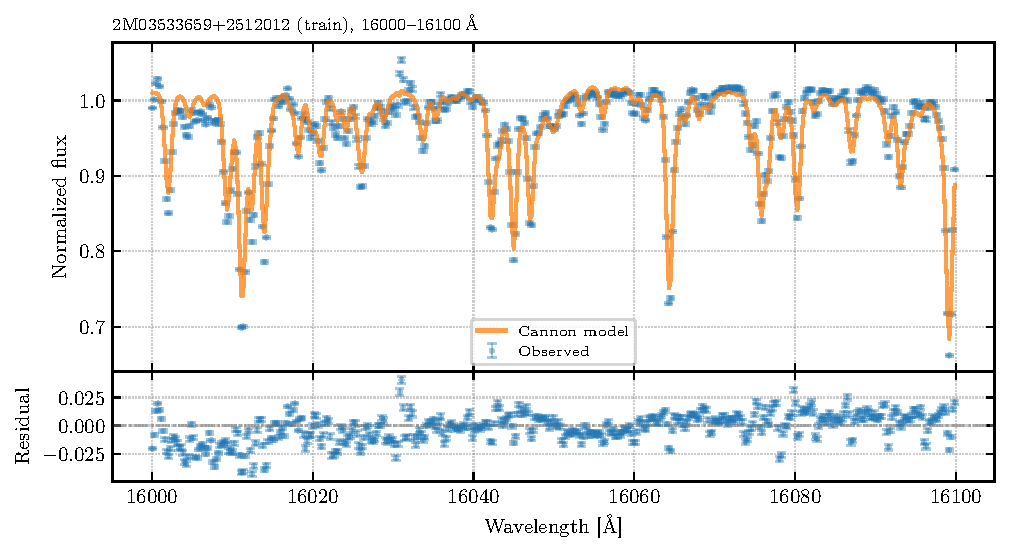
\includegraphics[width=\textwidth]{figures/fig_training_prediction.pdf}
  \caption{Training set prediction verification for star 2M03533659+2512012 in the wavelength range 16000--16100~\AA. \textit{Top:} Observed spectrum (blue) and Cannon-predicted spectrum (orange) are nearly indistinguishable. \textit{Bottom:} Residuals $(f_{\rm obs} - f_{\rm model})$ scatter around zero with standard deviation 0.013, comparable to the measurement uncertainty.}
  \label{fig:training_prediction}
\end{figure*}

\subsection{Gradient Spectra}
\label{sec:interpretation}

The gradient spectrum $\partial f_\lambda / \partial \ell_i$ quantifies the sensitivity of the flux at each wavelength to changes in label $\ell_i$. These are computed analytically from the polynomial coefficients $\boldsymbol{\theta}_\lambda$. Figure~\ref{fig:gradient_spectra} shows the gradient spectra for all five labels.

\begin{figure*}[b!]
  \centering
  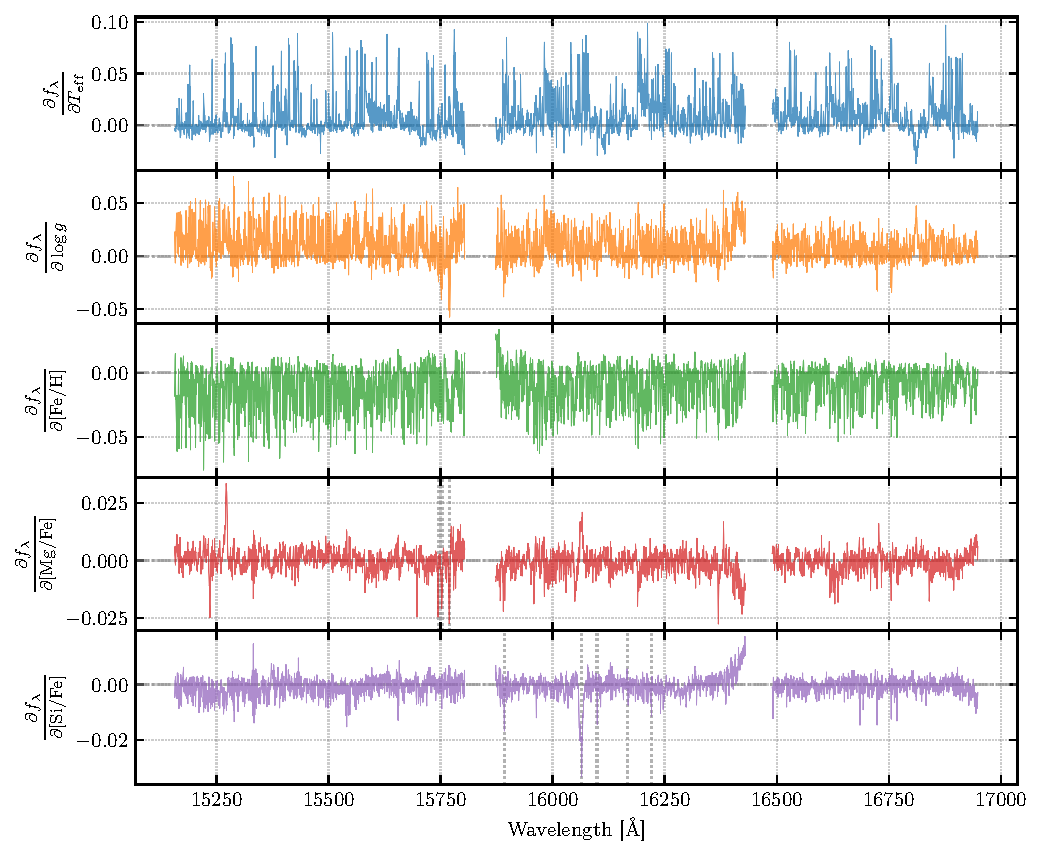
\includegraphics[width=\textwidth]{figures/fig_gradient_spectra.pdf}
  \caption{Gradient spectra $\partial f_\lambda / \partial \ell_i$ for each of the five labels. $T_{\rm eff}$ (top) shows a broadband response across the entire wavelength range, with the strongest features at CO molecular bands ($>$15580~\AA). $\log g$ shows pressure-broadened features. [Fe/H], [Mg/Fe], and [Si/Fe] show line-localized responses at known absorption features. Vertical markers on the [Mg/Fe] panel indicate known Mg~I lines (15741, 15749, 15765, 15879, 15886, 15954~\AA; \citealt{SmithApogee2013}); on the [Si/Fe] panel, known Si~I lines (15361, 15376, 15557, 15888, 15960, 16060, 16094, 16215, 16828~\AA).}
  \label{fig:gradient_spectra}
\end{figure*}

The $T_{\rm eff}$ gradient shows a broadband response where almost every pixel is sensitive to temperature, reflecting the Planck function's temperature dependence and possibly showing strong temperature sensitivity of unmodelled molecular bands as well. The strongest $T_{\rm eff}$ features correspond to CO bands $\sim$15580~\AA, where the molecular abundance is an exponential function of temperature.

The $\log g$ gradient is dominated by pressure-broadened features and hydrogen Brackett series lines, consistent with the role of surface gravity in setting the atmospheric pressure structure.

The abundance gradients ([Fe/H], [Mg/Fe], [Si/Fe]) are characteristically localized to sharp peaks at specific wavelengths corresponding to known absorption lines. On the [Mg/Fe] panel, the six Mg~I lines from \citet{SmithApogee2013} align with the strongest gradient features. Similarly, the nine Si~I lines appear prominently in the [Si/Fe] gradient. 

\subsection{Intrinsic Scatter Spectrum}

Figure~\ref{fig:scatter_spectrum} shows the per-pixel intrinsic scatter $s_\lambda$ as a function of wavelength.

\begin{figure*}[t!]
  \centering
  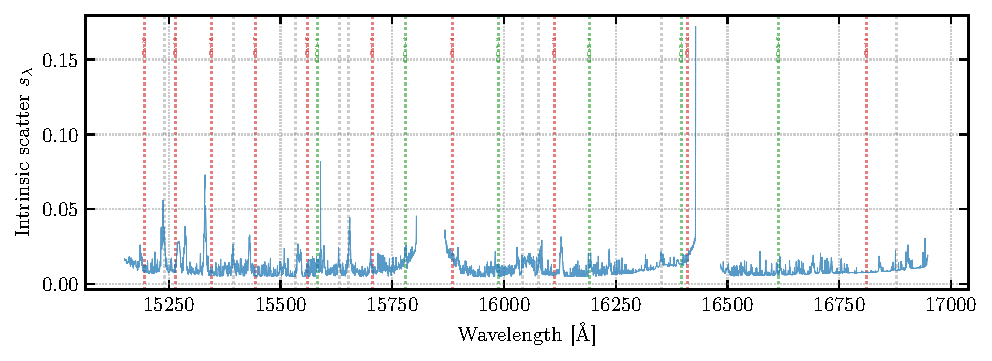
\includegraphics[width=\textwidth]{figures/fig_scatter_spectrum.pdf}
  \caption{Per-pixel intrinsic scatter $s_\lambda$ across the APOGEE wavelength range, with known absorption line positions indicated (Brackett series, CO bands, and atomic lines from Fe~I, Mg~I, Si~I, Al~I, Ca~I, Ti~I, Ni~I, K~I). High-scatter regions correspond to strong absorption lines where the second-order polynomial is insufficient to capture the full label dependence. Chip-edge artifacts also contribute elevated scatter at chip boundaries.}
  \label{fig:scatter_spectrum}
\end{figure*}

Broadly, regions of elevated scatter fall into three categories:
\begin{enumerate}
  \item Strong absorption lines where the flux depends nonlinearly on labels beyond second order.
  \item Chip-edge where pseudo-continuum normalization may be less reliable.
  \item Outlier-driven spikes stemming from isolated high-scatter pixels traceable to individual stars with anomalous features (e.g., emission lines, poor sky subtraction).
\end{enumerate}
Physically, a second-order polynomial in five labels has limited flexibility to capture the nonlinear dependence of line strength on temperature through the Boltzmann and Saha equations or Voigt profile shapes of strong lines; this can be visually observed in the example of Figure~\ref{fig:training_prediction}.

\subsection{Cross-Validation Label Recovery}
\label{sec:cv}

For each of the 944 stars in the CV set, we fit the five labels by minimizing $\chi^2$ (Eq.~\ref{eq:cannon_chi2}) using the TRF optimizer with analytical Jacobian. Figure~\ref{fig:label_recovery} shows the fitted labels vs.\ the ASPCAP reference values.

\begin{figure*}[t!]
  \centering
  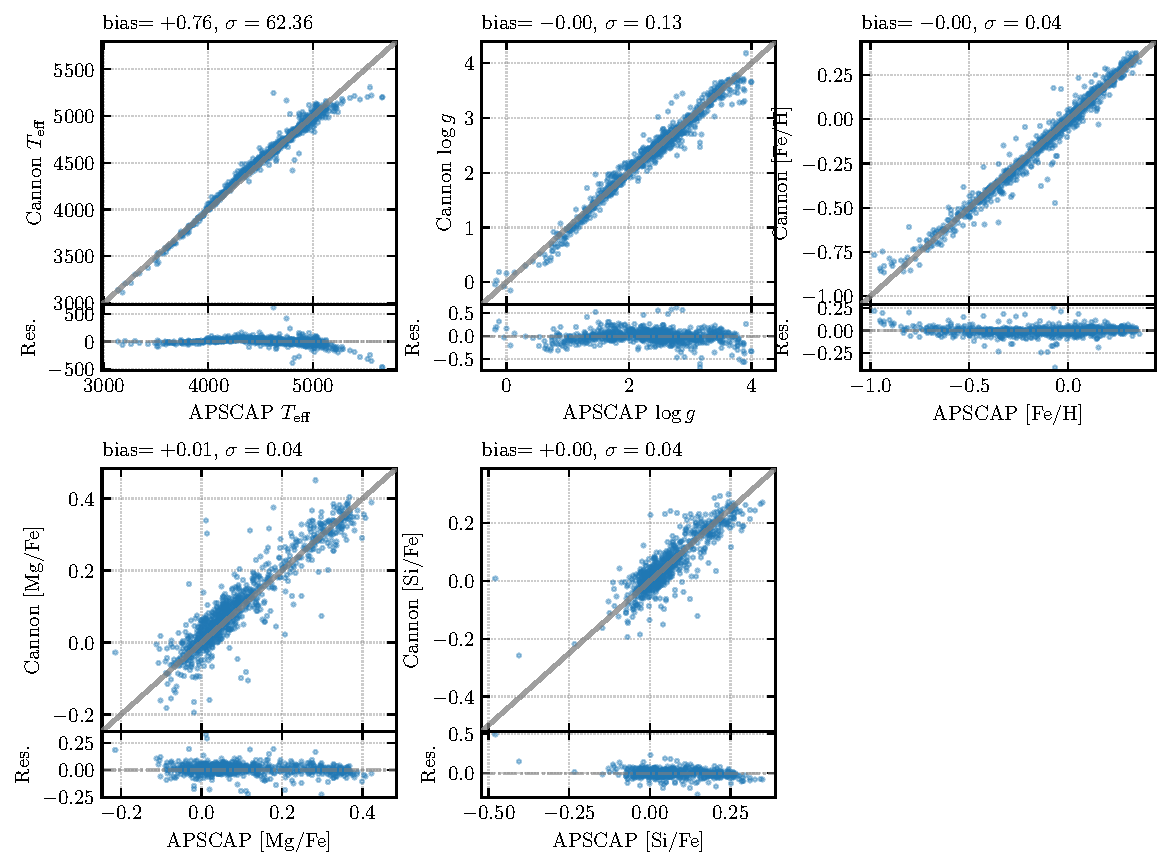
\includegraphics[width=\textwidth]{figures/fig_label_recovery.pdf}
  \caption{Cross-validation label recovery for 944 held-out stars. Each panel shows the Cannon-fitted label vs.\ the ASPCAP reference value, with a 1:1 line (dashed) and a residual sub-panel below. The three abundance labels ([Fe/H], [Mg/Fe], [Si/Fe]) are recovered with $\sim$0.04--0.05~dex scatter; $\log g$ at 0.13~dex; $T_{\rm eff}$ at 62~K scatter (the largest in absolute units but smallest in fractional terms, $\sim$1.3\%).}
  \label{fig:label_recovery}
\end{figure*}

Table~\ref{tab:cv_metrics} summarizes the bias and scatter for each label. All biases are negligible ($< 1$~K in $T_{\rm eff}$, $< 0.01$~dex in all others), confirming that the model is unbiased on average. The scatter values represent the fundamental precision floor of the Cannon model for this training set and polynomial order.

\begin{table}[H]
\centering
\caption{Cross-validation bias and scatter for each label.\label{tab:cv_metrics}}
\begin{tabular}{lcc}
\toprule
Label & Bias & Scatter ($1\sigma$) \\
\midrule
$T_{\rm eff}$ (K)   & $+0.8$   & 62.4  \\
$\log g$ (dex)       & $-0.004$ & 0.128 \\
$[\mathrm{Fe/H}]$ (dex) & $-0.004$ & 0.045 \\
$[\mathrm{Mg/Fe}]$ (dex) & $+0.008$ & 0.045 \\
$[\mathrm{Si/Fe}]$ (dex) & $+0.001$ & 0.044 \\
\bottomrule
\end{tabular}
\end{table}

We note that the lab manual suggests scatters of $\sim$30~K in $T_{\rm eff}$ and $\sim$0.02~dex in [Fe/H] ``should be achievable''; our global scatters exceed these by a factor of $\sim$2. For comparison, the original Cannon paper \citep{Ness2015} reported leave-one-out cross-validation scatters of $\sim$95.8~K in $T_{\rm eff}$, $\sim$0.24~dex in $\log g$, and $\sim$0.08~dex in [Fe/H] using 548 reference stars from cluster fields with only 3 labels. Our model substantially outperforms these values, likely due to the larger training set (942 stars), improved data quality in DR17 vs.\ DR10 and more feature-rich 5 labels. When we bin by $T_{\rm eff}$, the RGB core (4000--5000~K) achieves $\sim$40~K scatter, while the warm edge ($T_{\rm eff} > 5000$~K) degrades to 70--100~K due to polynomial saturation and less training stars. The global scatter is dominated by these hotter-end outliers. 

We intentionally do not apply outlier rejection to the CV metrics and report the more honest worse fit as it would be removing poorly-fit stars thus conflating model inadequacy and further reduce training coverage at the edges of label space where the model is already struggling.

\subsection{Outlier Investigation}

Figure~\ref{fig:outlier_spectra} contrasts the residuals $(f_{\rm obs} - f_{\rm model})$ for the three worst-fit and three best-fit CV stars (ranked by normalized label residual). The best-fit stars show residuals consistent with noise, while the worst-fit stars exhibit large spurious residual structures. Notably, the worst-fit residuals contain spurious peaks at the positions of strong absorption lines; these arise because the model predicts the wrong line depths, similar to the spectral features visible in the gradient spectra (Figure~\ref{fig:gradient_spectra}), confirming that the outliers are driven by label mismatch rather than instrumental artifacts.

\begin{figure}[t!]
  \centering
  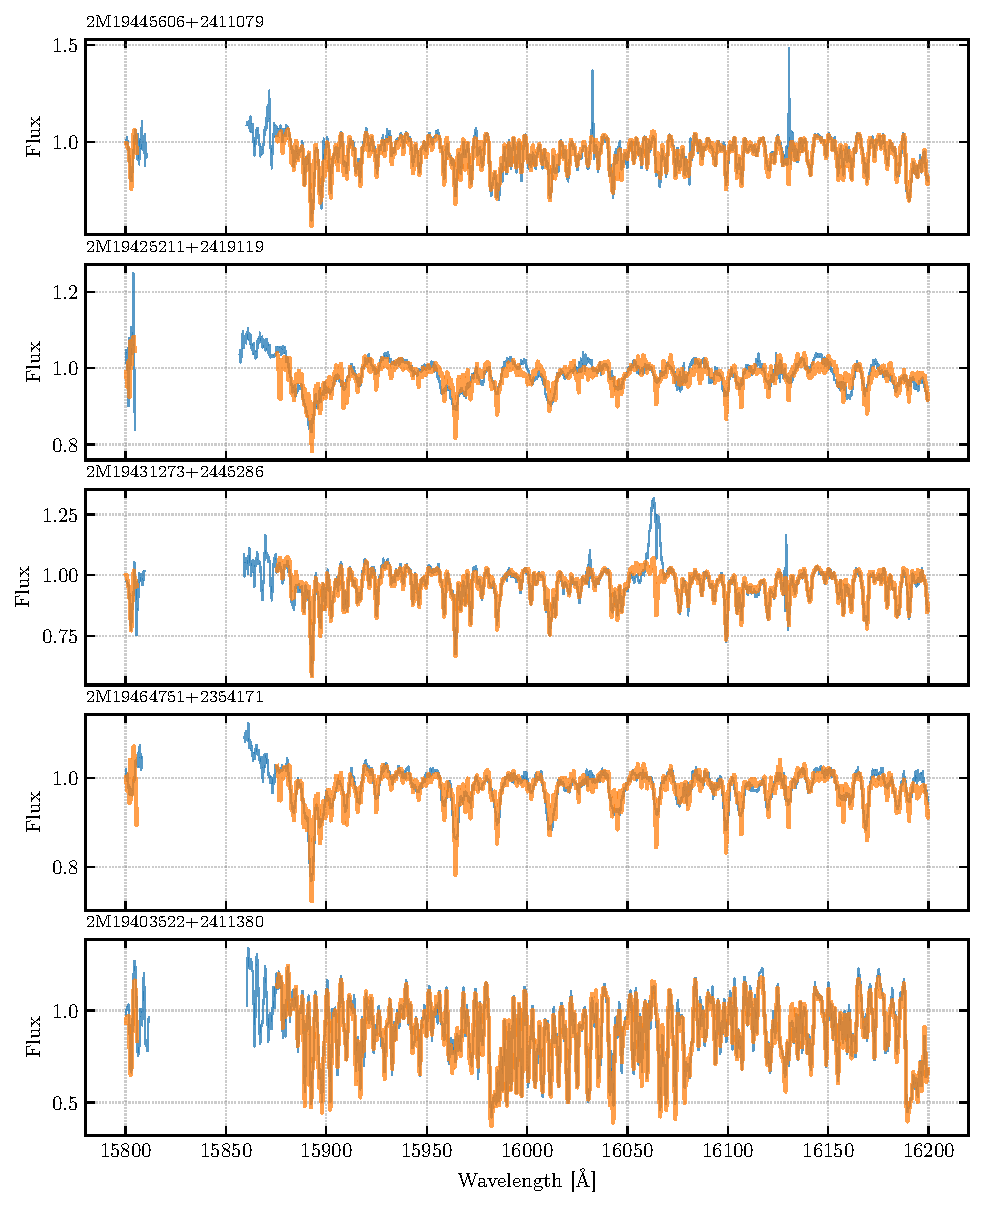
\includegraphics[width=\columnwidth]{figures/fig_outlier_spectra.pdf}
  \caption{Residuals $(f_{\rm obs} - f_{\rm model})$ in the 15800--16200~\AA\ window for the three worst-fit (\textit{top 3}, red) and three best-fit (\textit{bottom 3}, blue) cross-validation stars, ranked by normalized label residual. The best-fit stars have residuals consistent with measurement noise, confirming that the Cannon model accurately reproduces their spectra. The worst-fit stars show large, correlated residual structures at absorption line positions, indicating systematic model failure.}
  \label{fig:outlier_spectra}
\end{figure}

To address this and other possible drawbacks (e.g., poor pseudo-continuum normalization), The Cannon~2 \citep{Casey2016} introduces regularization via censoring and simultaneous pseudo-continuum normalization; we discuss these improvements further in Section~\ref{sec:future}.

%%% ---------------------------------------------------------------
\section{Neural Network Comparison}
\label{sec:nn}
%%% ---------------------------------------------------------------

\subsection{Architecture and Training}

As an alternative to The Cannon's forward-model-then-invert approach, we train MLPs (Section~\ref{sec:nn_theory}) to directly predict stellar labels from normalized spectra. We explore four architectures, summarized in Table~\ref{tab:nn_arch_specs}.

\begin{table*}[ht!]
\centering
\caption{Neural network architectures tested. All use ReLU activations. Parameter counts include biases.\label{tab:nn_arch_specs}}
\begin{tabular}{llrc}
\toprule
Variant & Layers & Parameters & Regularization \\
\midrule
Baseline & $8575 \to 512 \to 256 \to 5$ & 4,523,525 & None \\
Narrow (A) & $8575 \to 256 \to 128 \to 5$ & 2,228,741 & None \\
Deep (B) & $8575 \to 512 \to 256 \to 128 \to 5$ & 4,556,549 & None \\
Regularized (C) & $8575 \to 512 \to 256 \to 5$ & 4,523,525 & Dropout(0.3) + L2($10^{-4}$) \\
\bottomrule
\end{tabular}
\end{table*}

The baseline architecture (Eq.~\ref{eq:mlp_full}) uses two hidden layers of width 512 and 256, totaling 4,523,525 trainable parameters. Labels are normalized to zero mean and unit variance. Pixels with NaN or sentinel-valued uncertainties (masked and inter-chip-gap pixels) have their flux replaced with zero. The network is trained with MSE loss (Eq.~\ref{eq:mse_loss}) and the Adam optimizer \citep{Kingma2015} at learning rate $10^{-3}$, batch size 64, with early stopping (patience 20 epochs) on the validation loss.

The narrow variant (A) reduces both hidden layers to 256 and 128 units ($\sim$2.2M parameters), testing whether the baseline is over-parameterized for 942 training spectra. The deep variant (B) adds a third hidden layer ($512 \to 256 \to 128$), testing whether additional depth improves hierarchical feature extraction. The regularized variant (C) applies Dropout \citep{Srivastava2014} with $p = 0.3$ after each ReLU and L2 weight decay of $10^{-4}$ in the Adam optimizer, testing whether explicit regularization helps in the data-limited regime. All variants use the same training procedure (Adam, lr=$10^{-3}$, batch size 64, early stopping with patience 20).

\subsection{Training Diagnostics}

Figure~\ref{fig:nn_loss} shows the training and validation loss curves for the baseline architecture. Early stopping fires at epoch 85, with a train-validation gap of $\sim$10\%, indicating that rather than overfitting, the model has limited capacity to learn the features.

\begin{figure}[t!]
  \centering
  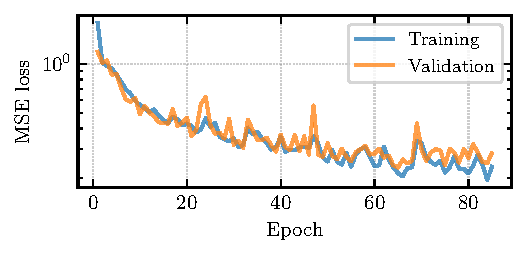
\includegraphics[width=\columnwidth]{figures/fig_nn_loss.pdf}
  \caption{Neural network training and validation MSE loss vs.\ epoch (log scale). The train-validation gap of $\sim$10\% indicates moderate underfitting due to limited capacity. Early stopping (patience 20) halted training at epoch 85.}
  \label{fig:nn_loss}
\end{figure}

\subsection{Label Recovery}

Figure~\ref{fig:nn_label_recovery} shows the NN label recovery on the CV set, and Table~\ref{tab:nn_comparison} compares the Cannon and baseline NN performance.

\begin{figure*}[t!]
  \centering
  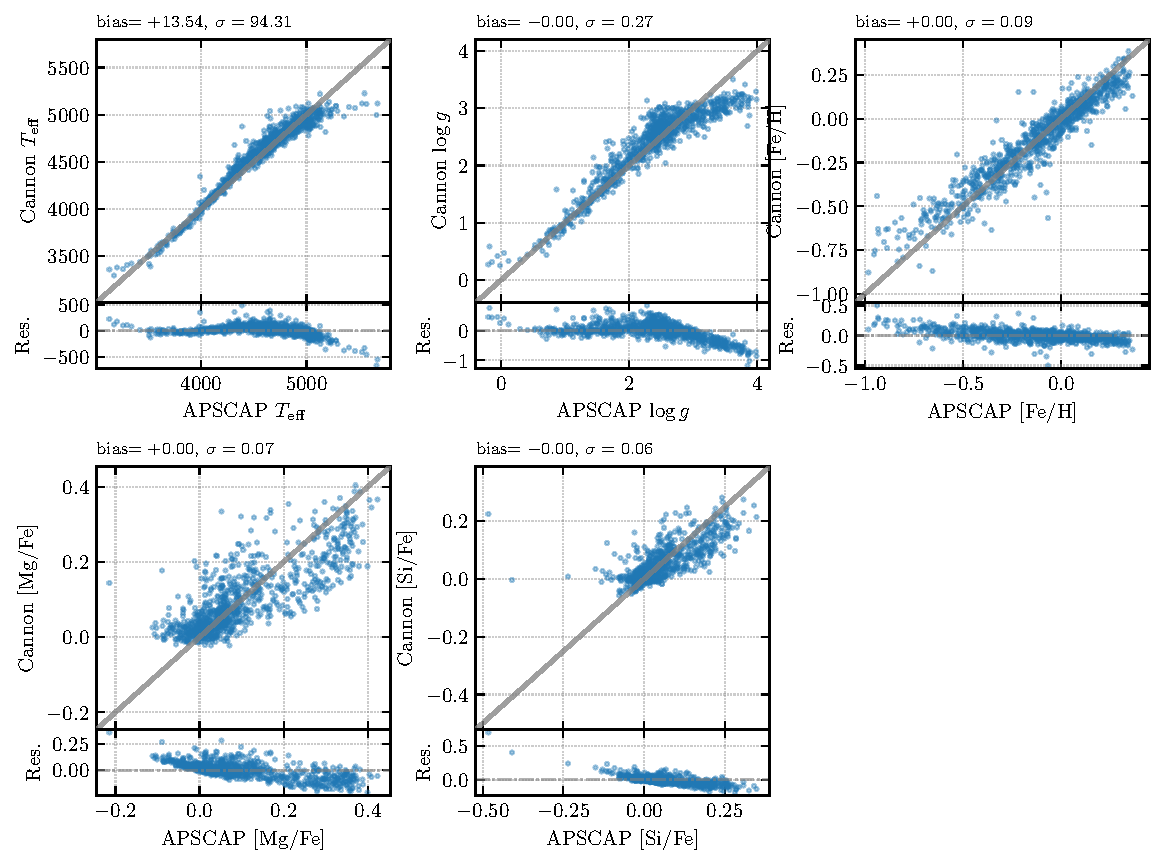
\includegraphics[width=\textwidth]{figures/fig_nn_label_recovery.pdf}
  \caption{Neural network label recovery for 944 cross-validation stars, in the same format as Figure~\ref{fig:label_recovery}. Compared to The Cannon, the scatter is $\sim$1.5--2$\times$ larger across all labels.}
  \label{fig:nn_label_recovery}
\end{figure*}

\begin{table*}[b!]
\centering
\caption{Performance comparison between The Cannon and the neural network on the cross-validation set.\label{tab:nn_comparison}}
\begin{tabular}{lcccccc}
\hline\hline
Label & Cannon bias & Cannon scatter & Cannon MAE & NN bias & NN scatter & NN MAE \\
\hline
$T_{\rm eff}$ (K)        & $+0.8$   & 62.4   & 24.3  & $+13.5$  & 94.3   & 48.3  \\
$\log g$ (dex)            & $-0.004$ & 0.128  & 0.062 & $-0.002$ & 0.265  & 0.144 \\
$[\mathrm{Fe/H}]$ (dex)  & $-0.004$ & 0.045  & 0.018 & $+0.000$ & 0.087  & 0.049 \\
$[\mathrm{Mg/Fe}]$ (dex) & $+0.008$ & 0.045  & 0.023 & $+0.000$ & 0.072  & 0.039 \\
$[\mathrm{Si/Fe}]$ (dex) & $+0.001$ & 0.044  & 0.020 & $-0.002$ & 0.058  & 0.025 \\
\hline\hline
\end{tabular}
\end{table*}

The Cannon outperforms the neural network on every label, with the NN scatter being 1.3--2.1$\times$ larger. First, The Cannon handles bad pixels naturally with bitmask-flagged pixels receiving inflated uncertainties ($\sigma > 10^6$) giving negligible weight in WLS training and $\chi^2$ fitting, while NaN-flux pixels propagate through and are excluded entirely; the NN instead receives zero-filled flux at masked pixels, which may introduce spurious features indistinguishable from physical absorption. Second, The Cannon's $\chi^2$ model takes into account varying per-pixel uncertainties, whereas the NN's MSE loss treats all pixels equally, giving equal weight to low SNR pixels. Thirdly, The Cannon is far more data-efficient with $\sim$22 parameters per pixel (21 coefficients + 1 scatter), each constrained by 942 training stars whereas the NN's 4.5M parameters trained on 942 spectra yield a $\sim$5000:1 parameter-to-datum ratio that makes overfitting a persistent risk even with early stopping. Finally, the second-order polynomial inherently encodes a physically motivated expectation of the data where spectral features are likely smoothly-varying, low-order functions of stellar labels. In contrast, NN has no such structural prior and must learn this from data alone.

\subsection{More Architectures}

Table~\ref{tab:nn_architectures} compares the CV scatter across all four architectures.

\begin{table*}[ht!]
\centering
\caption{CV scatter for alternative neural network architectures.\label{tab:nn_architectures}}
\begin{tabular}{lcccc}
\toprule
Label & Baseline & Narrow & Deep & Regularized \\
\midrule
$T_{\rm eff}$ (K)        & 94.3 & 84.1 & 85.4 & 175.3 \\
$\log g$ (dex)            & 0.265 & 0.244 & 0.239 & 0.387 \\
$[\mathrm{Fe/H}]$ (dex)  & 0.087 & 0.082 & 0.083 & 0.144 \\
$[\mathrm{Mg/Fe}]$ (dex) & 0.072 & 0.069 & 0.068 & 0.080 \\
$[\mathrm{Si/Fe}]$ (dex) & 0.058 & 0.056 & 0.054 & 0.062 \\
\bottomrule
\end{tabular}
\end{table*}

The narrow MLP ($8575 \to 256 \to 128 \to 5$) performs best among NN variants, achieving $\sim$10--20\% improvement over the baseline. This is consistent with the hypothesis that the 4.5M-parameter baseline is over-parameterized for 942 training spectra: reducing the parameter count by $\sim$2$\times$ forces the network to learn more efficient representations. The deep variant (B) performs similarly to the narrow variant, suggesting that additional depth does not help when the bottleneck is data quantity rather than model expressiveness. Adding explicit regularization (dropout + weight decay) performs worst, likely because the already-capacity-limited network cannot afford the additional reduction in effective capacity. Architecture tuning yields modest improvements, but The Cannon's structural advantage of $\sim$2$\times$ is not closed by any NN variant tested.

% \subsection{Advantages and Disadvantages}

% \begin{table*}[t]
% \centering
% \caption{Qualitative comparison of The Cannon and neural network approaches.\label{tab:comparison_qualitative}}
% \begin{tabular}{lll}
% \hline\hline
% Criterion & The Cannon & Neural Network \\
% \hline
% Interpretability & High: gradient spectra, per-pixel coefficients & Low: 4.5M opaque weights \\
% Uncertainty model & Explicit: per-pixel scatter + measurement error & None: MSE loss only \\
% Bad-pixel handling & Natural: inverse-variance weighting & Ad hoc: zero-filling \\
% Flexibility & Limited to 2nd-order polynomial & Arbitrary nonlinear mapping \\
% Training speed & $\sim$1 min (WLS per pixel) & $\sim$1 hr (GPU-accelerated) \\
% Inference speed & $\sim$1 s/star (optimization) & $\sim$1 ms/star (forward pass) \\
% Data efficiency & 22 params/pixel, well-constrained & 4.5M params, data-starved \\
% Scalability & Fixed polynomial order & Can absorb more data, labels \\
% \hline\hline
% \end{tabular}
% \end{table*}

% The Cannon excels in the low-data regime of this lab ($N \sim 1000$ training stars): its physically motivated polynomial basis provides a strong inductive prior that compensates for limited training data. The neural network would likely improve substantially with larger training sets ($N \gtrsim 10{,}000$), where its capacity to learn nonlinear features would become an advantage. For production surveys, physics-informed approaches such as The Payne \citep{Ting2019}, which uses a neural network to emulate ab initio spectral models, combine the interpretability of physical models with the flexibility of deep learning. Purely data-driven deep learning approaches such as astroNN \citep{Leung2019} can also achieve competitive performance when trained on large labeled datasets.

%%% ---------------------------------------------------------------
\section{Results and Discussion}
\label{sec:results}
%%% ---------------------------------------------------------------

We now apply the trained model to three further analyses: constructing a Kiel diagram to validate the fitted labels against stellar evolution theory, performing Bayesian MCMC fitting of an unknown stellar spectrum, and generating synthetic spectra to explore how metallicity and evolutionary state shape the $H$-band spectral morphology. We also discuss the systematic effects of unresolved binaries on label inference.

\subsection{Kiel Diagram and Stellar Evolution}
\label{sec:kiel}

Figure~\ref{fig:kiel_diagram} shows the Kiel diagram for the 944 CV stars, using the Cannon-fitted labels (not the ASPCAP reference values). Points are colored by fitted [Fe/H], and two MIST v2 isochrones \citep{Dotter2025}, solar metallicity ($[\mathrm{Fe/H}] = 0$) and metal-poor ($[\mathrm{Fe/H}] = -1$), both at an age of 6~Gyr, are overlaid.

\begin{figure*}[t!]
  \centering
  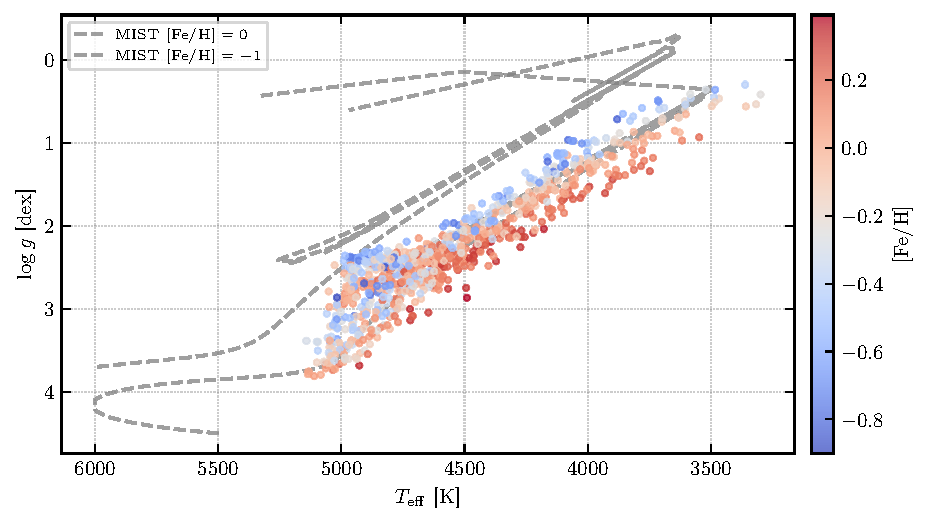
\includegraphics[width=\textwidth]{figures/fig_kiel_diagram.pdf}
  \caption{Kiel diagram ($\log g$ vs.\ $T_{\rm eff}$) for 944 cross-validation stars, colored by Cannon-fitted [Fe/H]. Overplotted are 6~Gyr MIST v2 isochrones at $[\mathrm{Fe/H}] = 0$ (solid) and $[\mathrm{Fe/H}] = -1$ (dashed). The red giant branch runs diagonally from lower-right (hot, high $\log g$) to upper-left (cool, low $\log g$). The red clump is visible as a dense concentration at $T_{\rm eff} \sim 4800$~K, $\log g \sim 2.5$. Metal-poor stars (blue points) are systematically hotter at fixed $\log g$, in agreement with the isochrone shift.}
  \label{fig:kiel_diagram}
\end{figure*}

The dominant structure is the red giant branch (RGB), a diagonal running from ($T_{\rm eff} \sim 5200$~K, $\log g \sim 3.5$) to ($T_{\rm eff} \sim 3800$~K, $\log g \sim 0.5$), traced by stars whose envelopes expand and cool as they ascend following hydrogen shell exhaustion. A dense concentration at $T_{\rm eff} \sim 4800$~K, $\log g \sim 2.5$ marks the red clump, population of core-helium-burning stars that have undergone the helium flash and settled onto a relatively stable burning phase.

A clear metallicity gradient is also visible: metal-poor stars ($[\mathrm{Fe/H}] < -0.5$, blue points) are systematically hotter at fixed $\log g$ than metal-rich stars ($[\mathrm{Fe/H}] > 0$, red points), reflecting the opacity effect in which lower metallicity reduces the envelope opacity and shifts the photosphere to higher temperatures at the same evolutionary state. The $[\mathrm{Fe/H}] = -1$ isochrone lies $\sim$200--400~K blueward of the solar isochrone at the same $\log g$, matching the observed shift. 

Together, the 6~Gyr MIST v2 isochrones trace the RGB morphology well, including the red-clump position and the base of the RGB, providing an independent validation that the Cannon-fitted labels are physically meaningful.

\subsection{Mystery Spectra}
\label{sec:mcmc}

\subsubsection{Setup and Priors}

We fit the mystery spectrum using MCMC described in Section~\ref{sec:theory}. The spectrum was processed through the same bitmask and normalization pipeline as the training data. We adopted the weakly informative Gaussian priors of Eq.~\eqref{eq:priors}, centered on the training-set means with widths of twice the training-set standard deviations.

\begin{figure*}[t!]
  \centering
  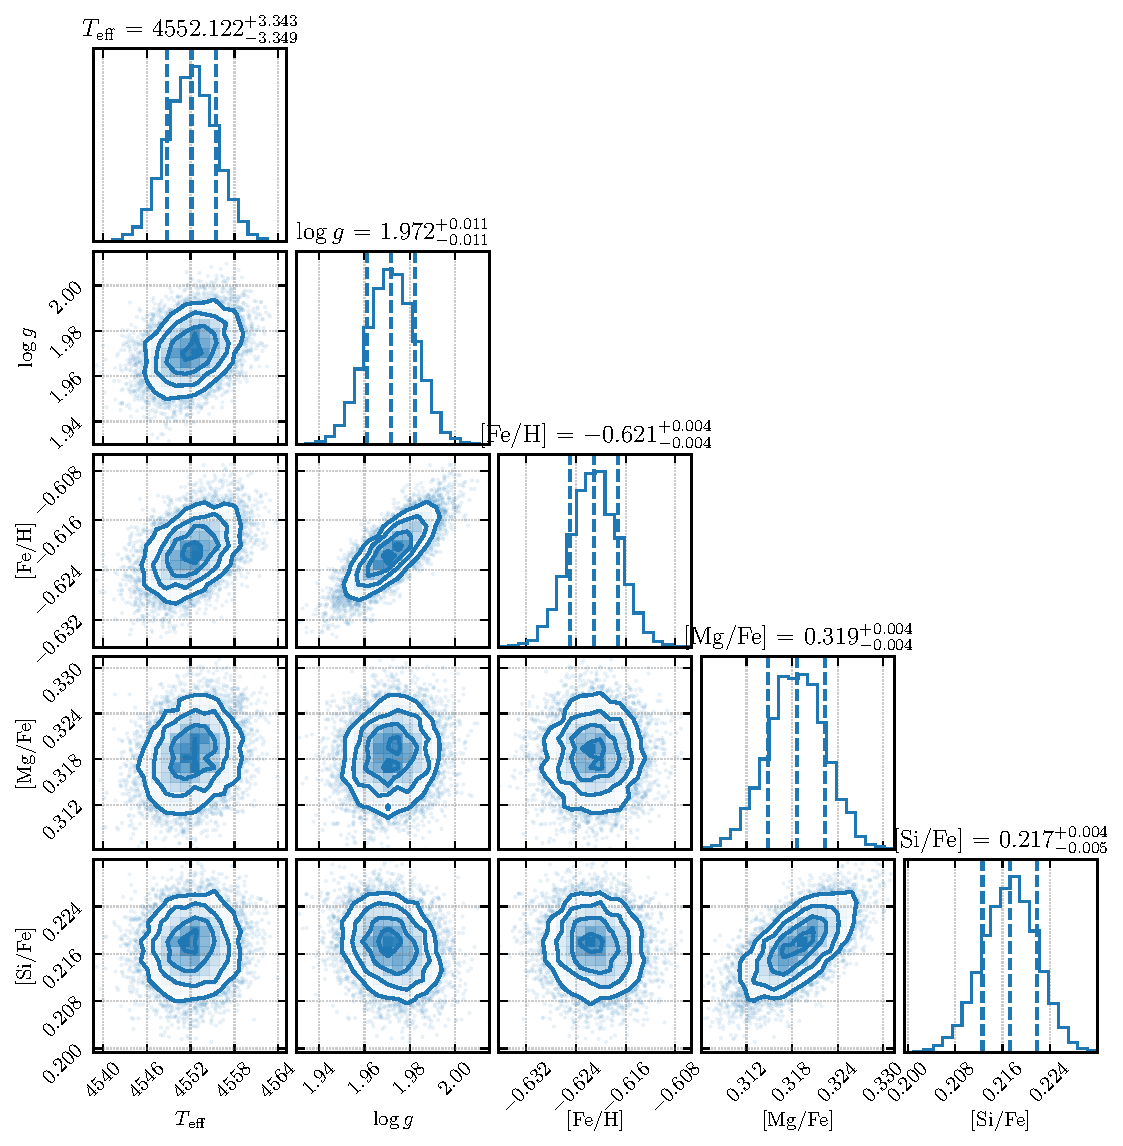
\includegraphics[width=\textwidth]{figures/fig_methods_corner.pdf}
  \caption{Corner plot of the MCMC posterior distribution for the mystery spectrum, showing the marginalized 1D and 2D projections of the five stellar labels. All parameters are tightly constrained, with the strongest correlation between $T_{\rm eff}$ and $\log g$.}
  \label{fig:methods_corner}
\end{figure*}

The MCMC was run with 4 chains $\times$ 2000 draws (after 1000 tuning steps each), totaling 8000 post-burn-in samples. All chains were initialized at the training-set mean labels. The trace plots (not shown) confirm that all four chains overlap with no stuck regions, and convergence with a 1000-step burn-in.

\subsubsection{Posterior Results}

Figure~\ref{fig:methods_corner} shows the corner plot of the posterior distribution over the five labels.

Table~\ref{tab:mcmc_results} gives the posterior medians and 68\% credible intervals.

The fitted $T_{\rm eff} \approx 4582$~K and $\log g \approx 1.99$ place the star within the red clump. The sub-solar metallicity $[\mathrm{Fe/H}] \approx -0.61$ is paired with strong $\alpha$-enhancement ($[\mathrm{Mg/Fe}] \approx +0.31$, $[\mathrm{Si/Fe}] \approx +0.21$), characteristic of old stellar populations whose chemical enrichment was dominated by core-collapse supernovae before Type~Ia supernovae contributed significant iron. Taken together, the chemical signature ($[\mathrm{Fe/H}] < -0.5$, $[\alpha/\mathrm{Fe}] > +0.2$) identifies the mystery star as an $\alpha$-enhanced red-clump giant consistent with membership in the Galactic thick disk or inner halo.

\subsubsection{Spectral Fit Quality}

Figure~\ref{fig:mystery_prediction} shows the observed mystery spectrum, the MCMC-predicted spectrum (evaluated at the posterior median labels), and the residuals.

\begin{figure*}[t!]
  \centering
  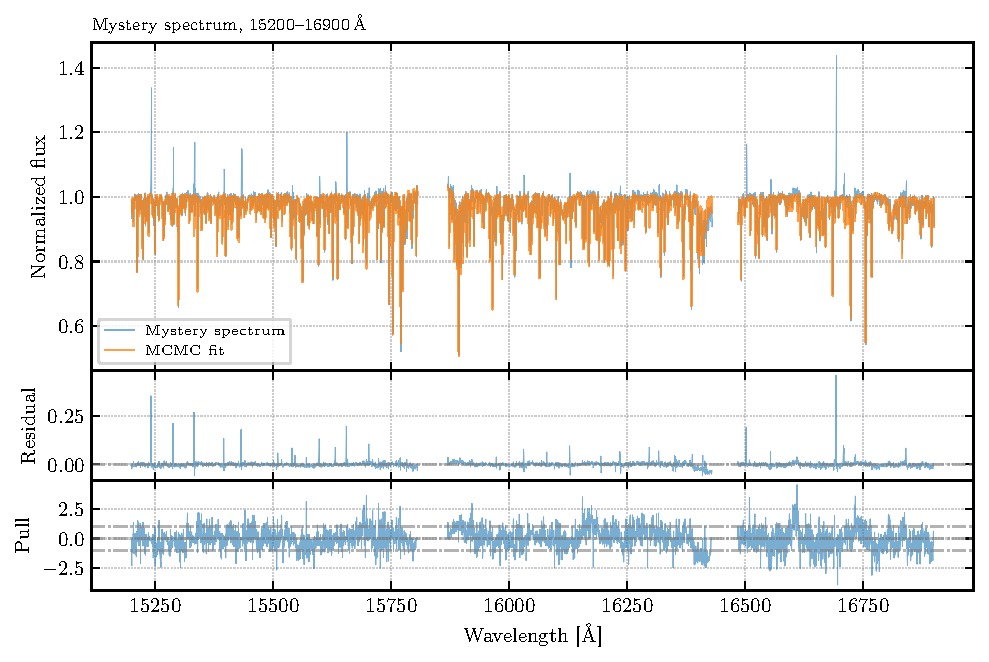
\includegraphics[width=\textwidth]{figures/fig_mystery_prediction.pdf}
  \caption{Mystery spectrum fit quality. \textit{Top:} Observed normalized spectrum with per-pixel error bars (blue) and MCMC-predicted spectrum at posterior median labels (orange). \textit{Bottom:} Residuals $(f_{\rm obs} - f_{\rm model})$ with error bars; the residuals scatter symmetrically around zero, confirming an adequate fit.}
  \label{fig:mystery_prediction}
\end{figure*}

\begin{table}[H]
\centering
\caption{MCMC posterior summary for the mystery spectrum (median $\pm$ 68\% credible interval half-width).\label{tab:mcmc_results}}
\begin{tabular}{lc}
\toprule
Label & Value \\
\midrule
$T_{\rm eff}$        & $4581.8 \pm 4.1$~K \\
$\log g$              & $1.989 \pm 0.010$~dex \\
$[\mathrm{Fe/H}]$    & $-0.610 \pm 0.004$~dex \\
$[\mathrm{Mg/Fe}]$   & $+0.315 \pm 0.005$~dex \\
$[\mathrm{Si/Fe}]$   & $+0.207 \pm 0.005$~dex \\
\bottomrule
\end{tabular}
\end{table}

The overall reduced $\chi^2_r = 0.60$ (computed with the total variance $\sigma_\lambda^2 + s_\lambda^2$ in the denominator) is slightly below unity, suggesting that the scatter term $s_\lambda^2$ slightly over-estimates the true model residuals for this particular star. Although this could just be a consequence of a good quality spectra being treated as overfitted by the scatter term trained on the full diversity of training-set stars, this could be symptomatic of the model potentially ovefitting.

\begin{table*}[b!]
\centering
\caption{Comparison of uncertainty estimates from three sources.\label{tab:uncertainty_comparison}}
\begin{tabular}{lccccc}
\hline\hline
Label & MCMC $\sigma$ & Cannon CV scatter & ASPCAP typical & CV/MCMC ratio \\
\hline
$T_{\rm eff}$ (K)        & 4.1  & 62.4  & $\sim$100 & 15.1 \\
$\log g$ (dex)            & 0.010 & 0.128 & $\sim$0.1 & 12.7 \\
$[\mathrm{Fe/H}]$ (dex)  & 0.004 & 0.045 & $\sim$0.05 & 11.0 \\
$[\mathrm{Mg/Fe}]$ (dex) & 0.005 & 0.045 & $\sim$0.03 & 8.9  \\
$[\mathrm{Si/Fe}]$ (dex) & 0.005 & 0.044 & $\sim$0.03 & 9.6  \\
\hline\hline
\end{tabular}
\end{table*}

\subsubsection{Uncertainty Discussion}

Table~\ref{tab:uncertainty_comparison} compares the MCMC uncertainties to the CV scatter (Section~\ref{sec:cv}) and typical ASPCAP errors \citep{Holtzman2015, Abdurrouf2022}.

The MCMC uncertainties are $\sim$10--15$\times$ smaller than the CV scatter. This discrepancy arises because the per-pixel scatter term $s_\lambda^2$ captures the variance of model residuals but cross-pixel model deviations (e.g., a poorly fit molecular band) which would contribute systematic label errors that are not reflected in the MCMC uncertainties. The CV scatter is therefore a more realistic estimate of the true label precision of the Cannon model. 

\subsection{Synthetic Spectra}
\label{sec:synthesis}

\subsubsection{Metallicity Sequence}

Figure~\ref{fig:metallicity_sequence} shows synthetic spectra generated by the trained Cannon model at fixed atmospheric parameters ($T_{\rm eff} = 4800$~K, $\log g = 2.5$, $[\mathrm{Mg/Fe}] = 0$, $[\mathrm{Si/Fe}] = 0$) with $[\mathrm{Fe/H}]$ varying from $-1.0$ to $+0.5$ in steps of 0.25~dex.

\begin{figure*}[t!]
  \centering
  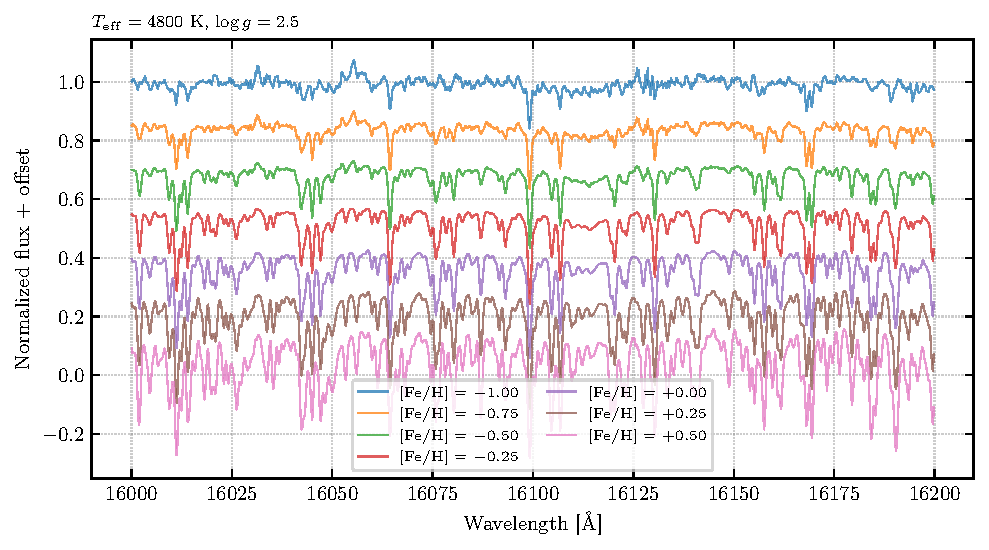
\includegraphics[width=\textwidth]{figures/fig_metallicity_sequence.pdf}
  \caption{Synthetic spectra at varying metallicity ($[\mathrm{Fe/H}] = -1.0$ to $+0.5$ in 0.25~dex steps), with fixed $T_{\rm eff} = 4800$~K, $\log g = 2.5$, $[\mathrm{Mg/Fe}] = 0$, $[\mathrm{Si/Fe}] = 0$. Spectra are vertically offset for clarity in the 16000--16200~\AA\ range. Fe~I absorption lines deepen monotonically with increasing [Fe/H], consistent with the curve of growth. The continuum level also decreases at high metallicity due to line blanketing (the cumulative opacity of millions of weak lines).}
  \label{fig:metallicity_sequence}
\end{figure*}

Several trends are visible. Fe~I absorption lines deepen monotonically with increasing [Fe/H]. At low abundance the lines are on the linear part and strengthen proportionally, while at higher abundance they saturate and broaden. The continuum level also decreases slightly at high metallicity due to line blanketing which is the cumulative opacity of millions of weak, unresolved lines. Notably, the spectral changes are highly localized to specific wavelengths, precisely the behavior captured by the line-localized [Fe/H] gradient spectrum (Figure~\ref{fig:gradient_spectra}).

\subsubsection{Red Giant Branch Evolution}

Figure~\ref{fig:rgb_evolution} shows synthetic spectra along the red giant branch, generated by sampling $\sim$7 points from a 6~Gyr, solar-metallicity MIST v2 isochrone \citep{Dotter2025} from $\log g = 3.5$ (base of the RGB) to $\log g = 0.5$ (near the tip), with $T_{\rm eff}$ varying self-consistently along the isochrone track.

\begin{figure*}[t]
  \centering
  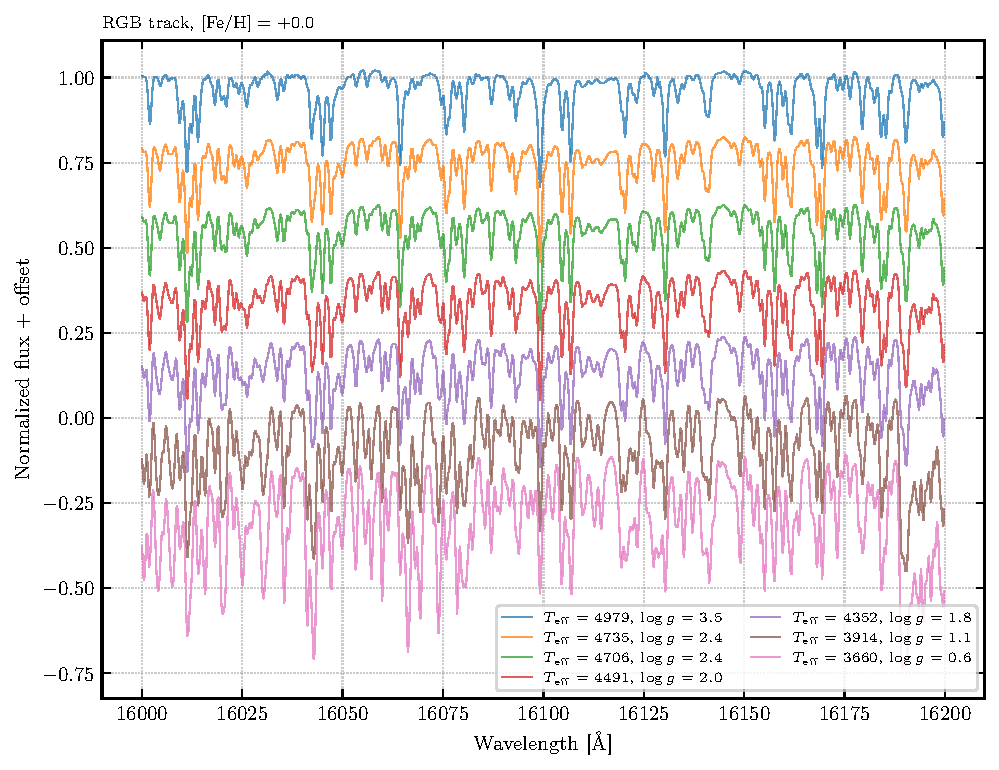
\includegraphics[width=\textwidth]{figures/fig_rgb_evolution.pdf}
  \caption{Synthetic spectra along the red giant branch at solar metallicity, sampled from a 6~Gyr MIST v2 isochrone ($\log g$ from 3.5 to 0.5, with $T_{\rm eff}$ varying self-consistently). Spectra are vertically offset for clarity. As the star ascends the RGB (decreasing $\log g$, decreasing $T_{\rm eff}$), absorption lines strengthen due to three coupled effects: Boltzmann/Saha ionization equilibrium shifts, pressure broadening weakens (lower $\log g$), and molecular bands (CO, OH) grow dramatically at low $T_{\rm eff}$.}
  \label{fig:rgb_evolution}
\end{figure*}

As $T_{\rm eff}$ decreases, the Boltzmann/Saha ionization equilibrium shifts from Fe~II toward Fe~I, strengthening neutral metal lines and altering the relative strengths of lines from different excitation levels. Simultaneously, the lower atmospheric pressure at reduced $\log g$ narrows pressure-broadened line profiles, partially counteracting the increased line strength from cooling. Most dramatically, CO and OH molecular abundances increase exponentially as $T_{\rm eff}$ drops below $\sim$4500~K; the CO first-overtone bands ($\lambda > 15580$~\AA) grow dramatically along the upper RGB, producing the most visually striking spectral changes.

\subsubsection{Sequence vs. Evolution}

Comparing Figures~\ref{fig:metallicity_sequence} and \ref{fig:rgb_evolution}, how can one tell the difference between a cool, low-$\log g$ star and a warmer, higher-$\log g$ star that is more metal-rich?

Metallicity changes predominantly affect metal lines (Fe~I, Mg~I, Si~I), scaling their equivalent widths roughly in proportion to abundance. Comparatively, RGB evolution, simultaneously changes the molecular band strengths (from temperature), pressure broadening (gravitationally), and ionization balance (affecting the ratio of neutral to ionized species). The Cannon model encodes this distinction in its gradient spectra (Figure~\ref{fig:gradient_spectra}) with the [Fe/H] gradient being localized to metal lines with near-zero response at CO bands, while the $T_{\rm eff}$ gradient has its largest features at the bands with a broadband component across all wavelengths as mentioned previously. This different label response breaks this degeneracy.

\subsection{Effects of Unresolved Binaries}
\label{sec:binaries}

Notably, the Cannon model does not take into account the presence of unresolved binary stars and assumes that the data is clean of unresolved binaries. If the angular separation between two components is smaller than the spectroscopic fiber diameter ($\sim$2\arcsec\ for APOGEE), the observed spectrum is a luminosity-weighted sum:
\begin{equation}
  f_\lambda^{\rm obs} = \frac{L_1}{L_1 + L_2} f_\lambda^{(1)} + \frac{L_2}{L_1 + L_2} f_\lambda^{(2)},
\end{equation}
where $f_\lambda^{(i)}$ are the individual normalized spectra and $L_i$ are the luminosities.

This composite spectrum does not correspond to any single point in label space, so the Cannon will fit intermediate labels that are biased relative to either component. In this case, the fitted $T_{\rm eff}$ is biased toward the luminosity-weighted average, typically higher than the primary's temperature because the secondary adds relatively more blue flux. For $\log g$, if both components are giants the bias is modest, but if one is a subgiant or main-sequence star $\log g$ may shift significantly. 

%%% ---------------------------------------------------------------
\section{Future Extensions}
\label{sec:future}
%%% ---------------------------------------------------------------

\subsection{Mitigating Unresolved Binary Contamination}

Several strategies could mitigate the effects of unresolved binaries (Section~\ref{sec:binaries}) on label inference: (1) fitting a two-component spectral model with separate label vectors for each star, allowing the optimizer to decompose the composite spectrum; (2) flagging likely binaries via radial velocity scatter across multiple APOGEE visits, since orbital motion produces measurable RV variations; and (3) identifying anomalous positions in the Kiel diagram.

\subsection{The Cannon 2 Improvements}

The Cannon~2 \citep{Casey2016} introduces several methodological improvements that could address the outlier categories identified in Section~\ref{sec:cannon}. Firstly, rather than fitting all pixels equally, The Cannon~2 downweights pixels known to be insensitive to a given label. This prevents the model from fitting noise in label-insensitive regions, reducing overfitting. Next, the current second-order polynomial becomes inadequate at strong, saturated absorption lines. A third-order model would add $\binom{5+3-1}{3} = 35$ cubic terms per pixel (56 total), potentially improving the fit at the cost of increased risk of overfitting with only 942 training stars. As such, the aforementioned censoring approach would required. Lastly, the continuum can only be trained as part of the model (rather than as a preprocessing step), which would eliminate the systematic errors introduced by imperfect normalization, which dominate the pixel-to-pixel correlations that inflate the MCMC uncertainty underestimate.

\subsection{Additional Improvements}

Crucially as mentioned before, the large scatters observed is symptomatic of the fact that the current training set spans only four APOGEE fields. Expanding to a larger, more diverse sample would improve coverage of the label space edges (particularly the warm $T_{\rm eff}$ boundary) and reduce the CV scatter.

Extending the model to include [C/Fe], [N/Fe], [Al/Fe], and other elements measured by ASPCAP would also make the model more physically meaningful. However, each additional label increases the number of polynomial terms, increasing the risk of overfitting once again.

%%% ---------------------------------------------------------------
\section{Conclusions}
\label{sec:conclusions}
%%% ---------------------------------------------------------------

We have constructed a data-driven spectral model for APOGEE DR17 red giants following The Cannon methodology \citep{Ness2015}. Starting from 1886 stars across four APOGEE fields, we trained a second-order polynomial model with 188,650 free parameters that achieves a training $\chi^2_r = 0.998$.

Cross-validation on 944 held-out stars demonstrates precisions of 62~K in $T_{\rm eff}$, 0.13~dex in $\log g$, 0.045~dex in [Fe/H], 0.045~dex in [Mg/Fe], and 0.044~dex in [Si/Fe], with negligible biases. Gradient spectra confirm that the model's learned features align with known atomic and molecular absorption lines, providing physical validation of the data-driven approach.

A Kiel diagram constructed from the Cannon-fitted labels recovers the expected stellar-evolutionary morphology---the red giant branch, the red clump, and the metallicity gradient---in good agreement with MIST v2 isochrone predictions. MCMC fitting of a mystery spectrum identifies it as a core-helium-burning, alpha-enhanced ($[\mathrm{Mg/Fe}] = +0.31$, $[\mathrm{Si/Fe}] = +0.21$) red-clump giant at sub-solar metallicity ($[\mathrm{Fe/H}] = -0.61$), consistent with a thick-disk or inner-halo origin. The MCMC uncertainties are $\sim$10--15$\times$ smaller than the empirical CV scatter, highlighting the importance of unmodelled pixel-to-pixel correlations in spectroscopic uncertainty budgets.

Synthetic spectra illustrate that metallicity changes produce localized line-strength variations, while RGB evolutionary changes produce coupled temperature, pressure, and molecular effects across the full spectral range. These distinct spectral ``fingerprints'' allow the model to break the temperature-metallicity degeneracy. The effects of unresolved binary contamination on spectral label inference are discussed, with biases toward intermediate temperatures and diluted abundances.

A neural network comparison demonstrates that The Cannon's physically motivated polynomial basis provides a strong inductive prior in the data-limited regime ($N \sim 1000$), outperforming a 4.5M-parameter MLP by $\sim$1.5--2$\times$ on all labels. Future work could combine the strengths of both approaches through hybrid physics-informed neural networks.

\section*{Acknowledgements}
Special thanks to Prof. Joshua Bloom and GSI Saahit Mogan for instructional support.
I also acknowledge the use of Claude Code for assistance
with vetting phrasing and checking the report writeup.

\bibliographystyle{aasjournal}
\bibliography{references}

\appendix

\section{Reproducibility Notes}

All code, notebooks, cached analysis products, and report sources used for this lab are version-controlled at \url{https://github.com/raw-asparagus/ay-128}.

\end{document}
